% GovAllocXAI -- JOURNAL manuscript, single-column article layout (blue headings, A4, Times).
% Compiles with pdfLaTeX: pdflatex, bibtex, pdflatex x2. The body is class-independent; swap the preamble for a journal class if the target journal requires its own template.
\PassOptionsToPackage{hyphens}{url}
\documentclass[11pt,a4paper]{article}
\usepackage[T1]{fontenc}
\usepackage[utf8]{inputenc}
\usepackage{mathptmx}
\usepackage[a4paper,left=2.6cm,right=2.6cm,top=2.6cm,bottom=2.8cm]{geometry}
\usepackage{microtype}
\usepackage{amsmath,amssymb}
\usepackage{graphicx,booktabs,xcolor}
\usepackage{enumitem}
\usepackage[section]{placeins}
\usepackage{titlesec}
\definecolor{linkblue}{RGB}{0,82,164}
\titleformat{\section}{\Large\bfseries\color{linkblue}}{\thesection.}{0.6em}{}
\titleformat{\subsection}{\large\bfseries\color{linkblue}}{\thesubsection}{0.6em}{}
\titleformat{\subsubsection}{\normalsize\bfseries\color{linkblue}}{\thesubsubsection}{0.6em}{}
\titlespacing*{\section}{0pt}{2.2ex plus 1ex minus .2ex}{1.2ex plus .2ex}
\titlespacing*{\subsection}{0pt}{1.8ex plus 1ex minus .2ex}{0.9ex plus .2ex}
\usepackage{cite}
\usepackage{url}
\usepackage[colorlinks=true,linkcolor=linkblue,citecolor=linkblue,urlcolor=linkblue]{hyperref}
\Urlmuskip=0mu plus 2mu
\emergencystretch=3em
\linespread{1.07}
\setlength{\parskip}{4pt plus 1pt}
\makeatletter\renewcommand{\fps@table}{htbp}\expandafter\def\csname fps@table*\endcsname{htbp}\makeatother
% Macros regenerated by pipeline/27_make_figures_tables.py - do not edit by hand
\newcommand{\NMasterRows}{5{,}450}
\newcommand{\NMasterCols}{217}
\newcommand{\NMasterCountries}{217}
\newcommand{\NCofogRows}{825}
\newcommand{\NCofogCountries}{36}
\newcommand{\NWdiRows}{4{,}995}
\newcommand{\NWdiCountries}{211}
\newcommand{\NLegacyMatched}{750}
\newcommand{\NOecdAdded}{6}
\newcommand{\NOecdRowsComplete}{109}
\newcommand{\NOverlapRows}{690}
\newcommand{\NXsrcMedDiff}{0.025}
\newcommand{\NXsrcMinR}{0.996}
\newcommand{\NWdiIndicators}{26}
\newcommand{\NFeatNum}{30}
\newcommand{\NFeatModel}{25}
\newcommand{\NSlsqpDiff}{3.6e-15}
\newcommand{\ResTVDPersist}{3.62}
\newcommand{\ResTVDPersistLo}{3.17}
\newcommand{\ResTVDPersistHi}{4.08}
\newcommand{\ResTVDHyb}{3.48}
\newcommand{\ResTVDHybLo}{3.06}
\newcommand{\ResTVDHybHi}{3.91}
\newcommand{\ResTVDCountryMean}{6.96}
\newcommand{\ResPairedGain}{0.140}
\newcommand{\ResPairedLo}{0.025}
\newcommand{\ResPairedHi}{0.277}
\newcommand{\ResRowsImproved}{53}
\newcommand{\ResColdHyb}{10.77}
\newcommand{\ResColdHybLo}{9.60}
\newcommand{\ResColdHybHi}{12.05}
\newcommand{\ResColdPeer}{11.34}
\newcommand{\ResColdGlobal}{11.35}
\newcommand{\ResColdGain}{0.35}
\newcommand{\ResColdGainLo}{-0.44}
\newcommand{\ResColdGainHi}{1.10}
\newcommand{\ATest}{178}
\newcommand{\ATrain}{611}
\newcommand{\AYearLo}{2000}
\newcommand{\AYearHi}{2024}
\newcommand{\LegXGBR}{0.996}
\newcommand{\LegFormulaR}{0.924}
\newcommand{\LegConstRatioR}{-0.011}
\newcommand{\LegNConst}{11}
\newcommand{\LegNIdent}{12}
\newcommand{\LegHealthWith}{0.987}
\newcommand{\LegHealthWithout}{0.969}
\newcommand{\LegTempXGB}{0.945}
\newcommand{\LegTempFormula}{0.932}
\newcommand{\EngTVDBefore}{3.48}
\newcommand{\AgrHealthRho}{0.58}
\newcommand{\AgrSocialProtectionRho}{0.64}
\newcommand{\AgrDefenceRho}{0.52}
\newcommand{\AgrEducationRho}{0.67}
\newcommand{\AgrTransportRho}{0.59}
\newcommand{\AgrGeneralPublicServicesRho}{0.56}
\newcommand{\AgrRhoMean}{0.59}
\newcommand{\AgrJacMean}{0.48}
\newcommand{\AgrSignMean}{0.85}
\newcommand{\AgrLimeFit}{0.52}
\newcommand{\AgrStabMean}{0.86}
\newcommand{\AgrFaithMean}{3.1}
\newcommand{\AgrFaithMin}{2.0}
\newcommand{\AgrFaithMax}{3.8}
\newcommand{\LegXGBRConst}{0.9991}
\newcommand{\LegFormulaRConst}{0.9997}
\newcommand{\LegRealXGB}{0.987}
\newcommand{\LegRealFormula}{0.714}
\newcommand{\LegConstRatioConst}{-0.0002}
\newcommand{\LegXGBRatioConst}{0.88}
\newcommand{\FSStackTenGain}{1.26}
\newcommand{\FSStackTenLo}{0.68}
\newcommand{\FSStackTenHi}{1.84}
\newcommand{\FSStackTenHolm}{0.0008}
\newcommand{\FSStackSixteenGain}{0.81}
\newcommand{\FSStackSixteenLo}{0.20}
\newcommand{\FSStackSixteenHi}{1.34}
\newcommand{\FSStackSixteenHolm}{0.060}
\newcommand{\FSXgbTenGain}{0.89}
\newcommand{\FSXgbTenLo}{0.19}
\newcommand{\FSXgbTenHi}{1.58}
\newcommand{\FSXgbTenHolm}{0.060}
\newcommand{\FSXgbSixteenGain}{0.47}
\newcommand{\FSXgbSixteenLo}{-0.22}
\newcommand{\FSXgbSixteenHi}{1.13}
\newcommand{\FSXgbSixteenHolm}{0.171}
\newcommand{\FSKnnTenGain}{1.25}
\newcommand{\FSKnnTenLo}{0.71}
\newcommand{\FSKnnTenHi}{1.78}
\newcommand{\FSKnnTenHolm}{0.0008}
\newcommand{\FSKnnSixteenGain}{0.66}
\newcommand{\FSKnnSixteenLo}{0.19}
\newcommand{\FSKnnSixteenHi}{1.14}
\newcommand{\FSKnnSixteenHolm}{0.034}
\newcommand{\FSStackXgbTenGain}{0.38}
\newcommand{\FSStackXgbTenLo}{0.06}
\newcommand{\FSStackXgbTenHi}{0.69}
\newcommand{\FSStackXgbTenHolm}{0.060}
\newcommand{\FSStackXgbSixteenGain}{0.34}
\newcommand{\FSStackXgbSixteenLo}{-0.03}
\newcommand{\FSStackXgbSixteenHi}{0.71}
\newcommand{\FSStackXgbSixteenHolm}{0.140}
\newcommand{\FSTVDPeerTen}{14.99}
\newcommand{\FSTVDStackTen}{13.73}
\newcommand{\FSTVDKnnTen}{13.74}
\newcommand{\FSTVDPeerSixteen}{11.31}
\newcommand{\FSTVDStackSixteen}{10.50}
\newcommand{\ResidualMean}{2.6}
\newcommand{\ResidualMedian}{1.8}
\newcommand{\ResidualMax}{29.7}
\newcommand{\AnnSeedMeanGain}{0.12}
\newcommand{\AnnSeedMinGain}{0.10}
\newcommand{\AnnSeedMaxGain}{0.14}
\newcommand{\AnnSeedNExcl}{1}
\newcommand{\AnnSeedN}{5}
\newcommand{\AnnXgbSeedMeanGain}{0.04}
\newcommand{\CovPooledHealth}{0.41}
\newcommand{\CovPooledSocial}{0.31}
\newcommand{\CovPooledEducation}{0.51}
\newcommand{\CovTwentyHealth}{0.27}
\newcommand{\CovTwentySocial}{0.34}
\newcommand{\NTenRows}{1526}
\newcommand{\NTenEcon}{85}
\newcommand{\NTenImf}{623}
\newcommand{\ColdStackSixteen}{10.53}
\newcommand{\ColdPeerSixteen}{11.34}
\newcommand{\ColdStackTen}{13.77}
\newcommand{\ColdStackTenLo}{12.30}
\newcommand{\ColdStackTenHi}{15.45}
\newcommand{\ColdPeerTen}{15.01}
\newcommand{\ColdBestTen}{14.12}
\newcommand{\HistPersistTen}{4.62}
\newcommand{\HistStackTen}{4.82}
\newcommand{\HistBestTen}{4.56}
\newcommand{\NovRho}{0.70}
\newcommand{\ErrHigh}{11.4}
\newcommand{\ErrLow}{33.4}
\newcommand{\ErrLowerMid}{22.0}
\newcommand{\HistStackSixteen}{3.50}
\newcommand{\TotPersist}{2.87}
\newcommand{\TotDeltaRidge}{1.83}
\newcommand{\TotColdMean}{5.63}
\newcommand{\TotColdRidge}{3.82}

% All figure environments (journal). Each figure is a macro that is called once, next to the text that first discusses it.
% Conference version: figs_conf.tex.
\newcommand{\figArch}{\begin{figure}[htbp]
\centering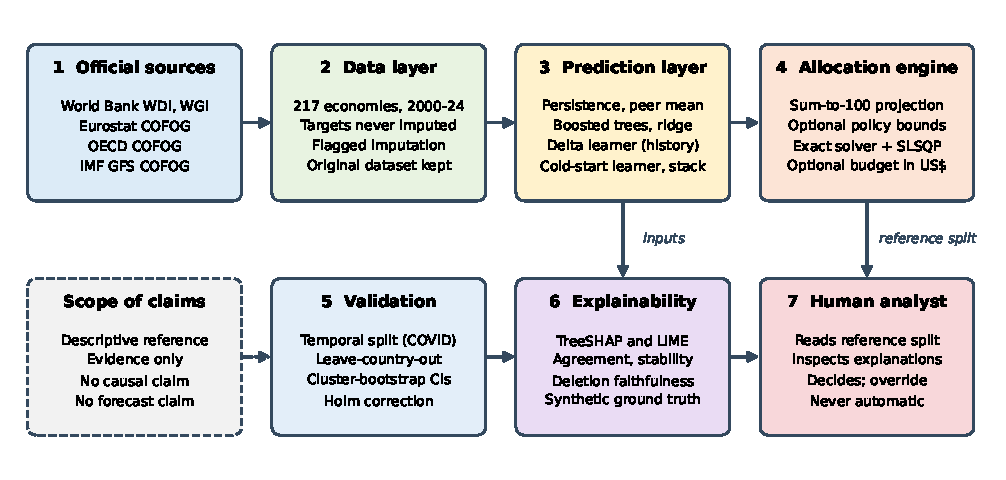
\includegraphics[width=\textwidth]{figures/fig1_architecture.pdf}
\caption{Evaluated components of GovAllocXAI. Official sources feed a flagged data layer; the prediction layer offers a history-based $\Delta$-learner and a cold-start peer learner; a bounded-simplex projection enforces the budget identity and optional bounds; explanations and a validation protocol surround every prediction; the intended user is a human analyst.}\label{fig:arch}
\end{figure}}
\newcommand{\figCoverage}{\begin{figure}[htbp]
\centering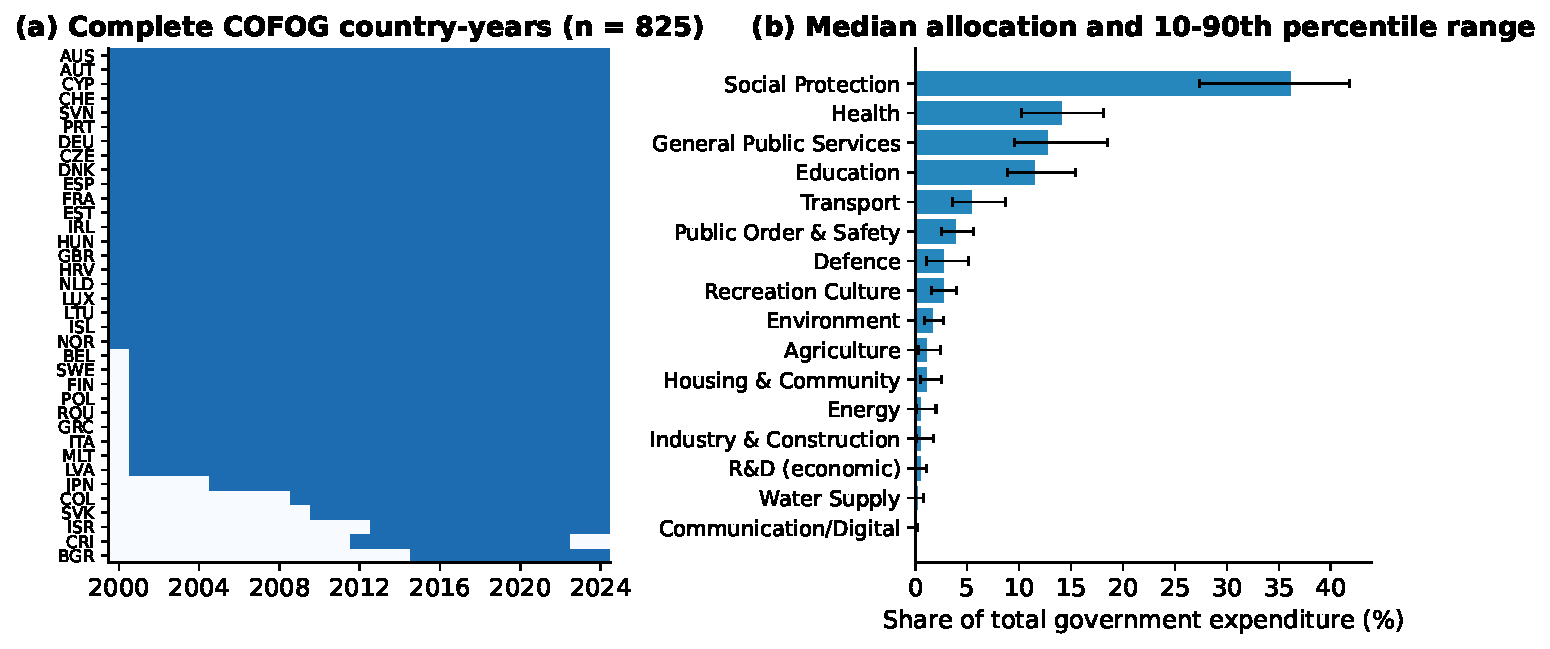
\includegraphics[width=\textwidth]{figures/fig2_data_coverage.pdf}
\caption{Data (panel A16). (a) Country-years with a complete 16-function COFOG breakdown (Eurostat for EU/EFTA, OECD otherwise). (b) Median share of total government expenditure per function with 10th--90th percentile range.}\label{fig:coverage}
\end{figure}}
\newcommand{\figAudit}{\begin{figure}[htbp]
\centering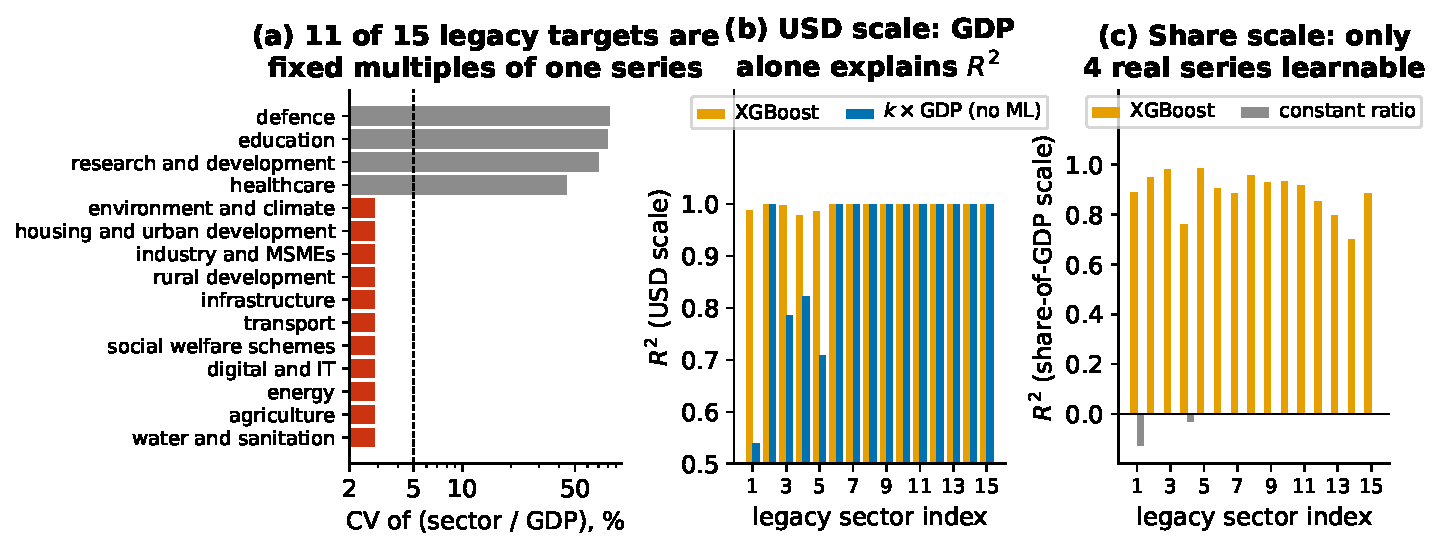
\includegraphics[width=\textwidth]{figures/fig3_legacy_audit.pdf}
\caption{Forensic audit of the legacy v1 benchmark ($n=775$ rows). (a) Coefficient of variation of sector/GDP: eleven sectors are below 5\% (they are exact multiples of one series). (b) On the USD scale a rule $k\times$GDP matches XGBoost on those sectors. (c) On the share-of-GDP scale a constant predictor has $R^2\approx0$ on them. Sector indices follow Table~\ref{tab:audit}.}\label{fig:audit}
\end{figure}}
\newcommand{\figMain}{\begin{figure}[htbp]
\centering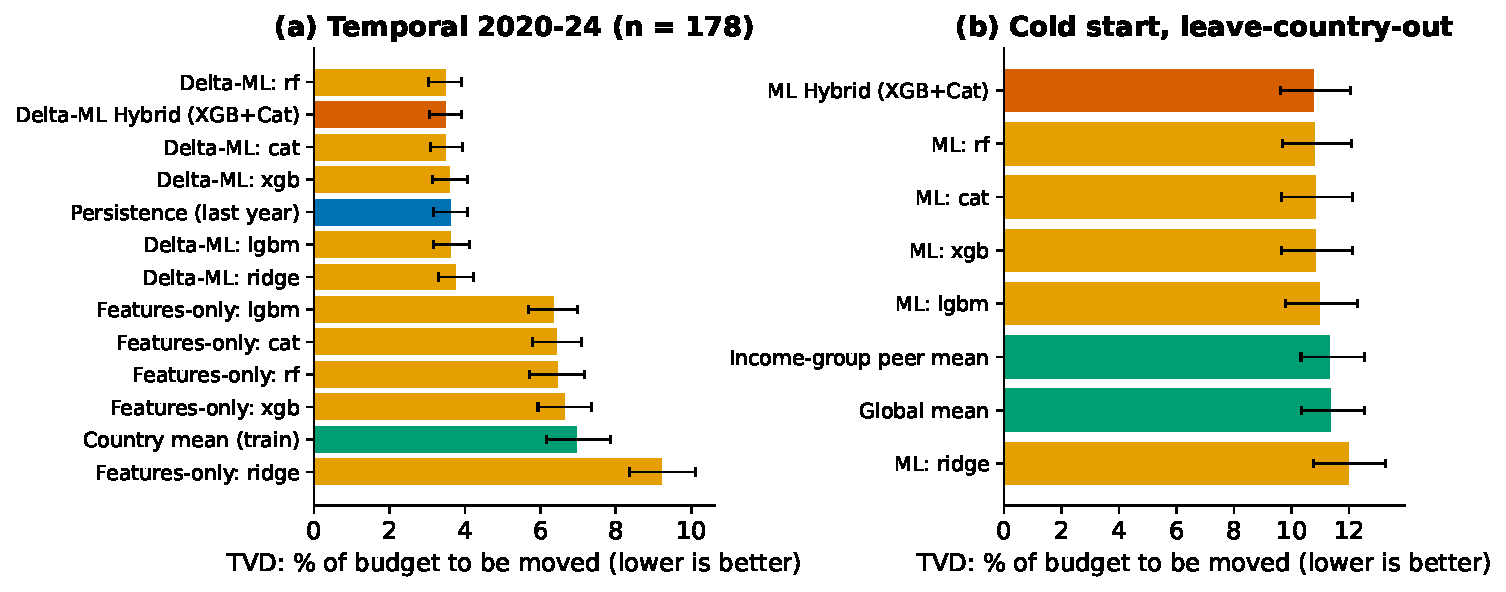
\includegraphics[width=\textwidth]{figures/fig4_main_results.pdf}
\caption{Main results on panel A16 (lower TVD is better; bars show 95\% cluster-bootstrap CIs). (a) Annual update, test 2020--24 ($n=178$): persistence is hard to beat. (b) Cold start, 825 country-years, two fold seeds: boosted learners vs.\ peer and global means.}\label{fig:main}
\end{figure}}
\newcommand{\figPerfn}{\begin{figure}[htbp]
\centering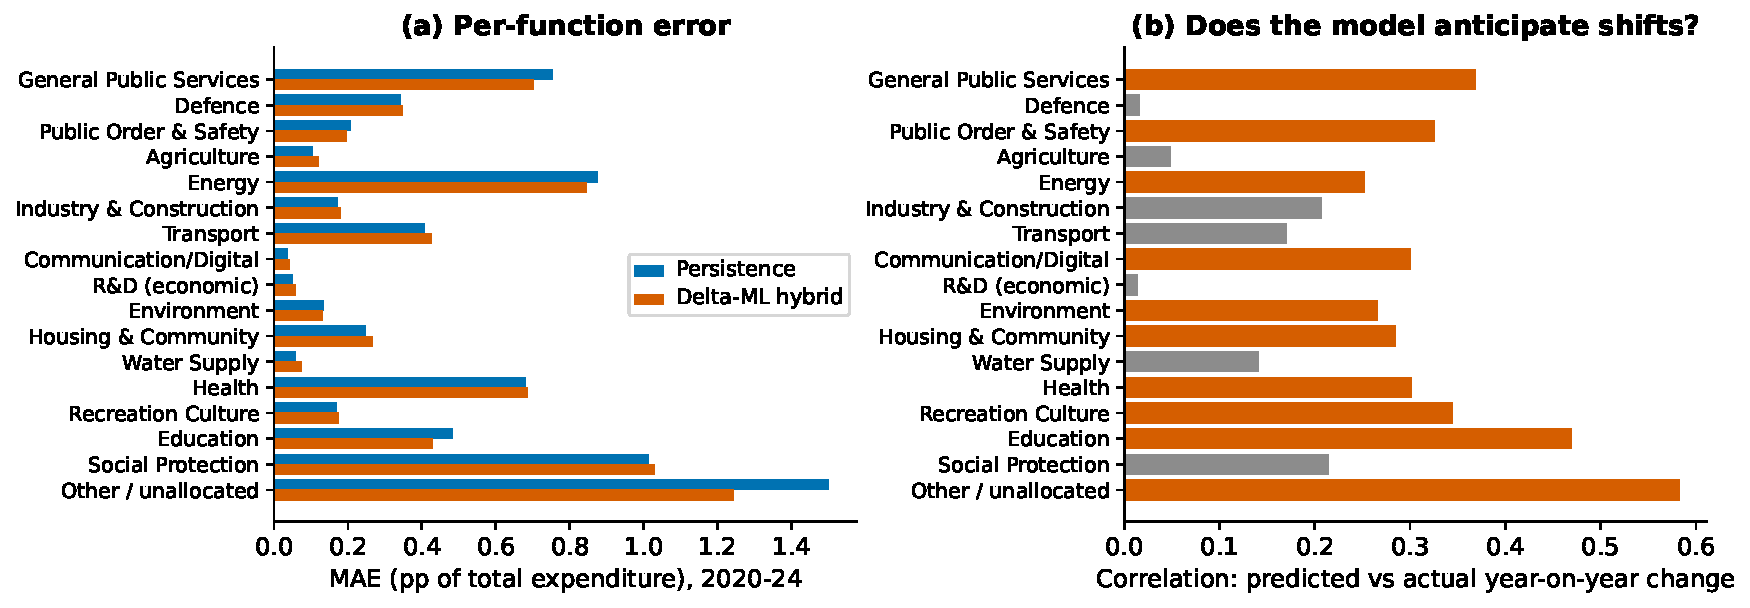
\includegraphics[width=\textwidth]{figures/fig5_per_function.pdf}
\caption{(a) Per-function error of persistence and the $\Delta$-hybrid on the 2020--2024 test window ($n=178$). (b) Correlation between predicted and observed year-on-year changes.}\label{fig:perfn}
\end{figure}}
\newcommand{\figWdi}{\begin{figure}[htbp]
\centering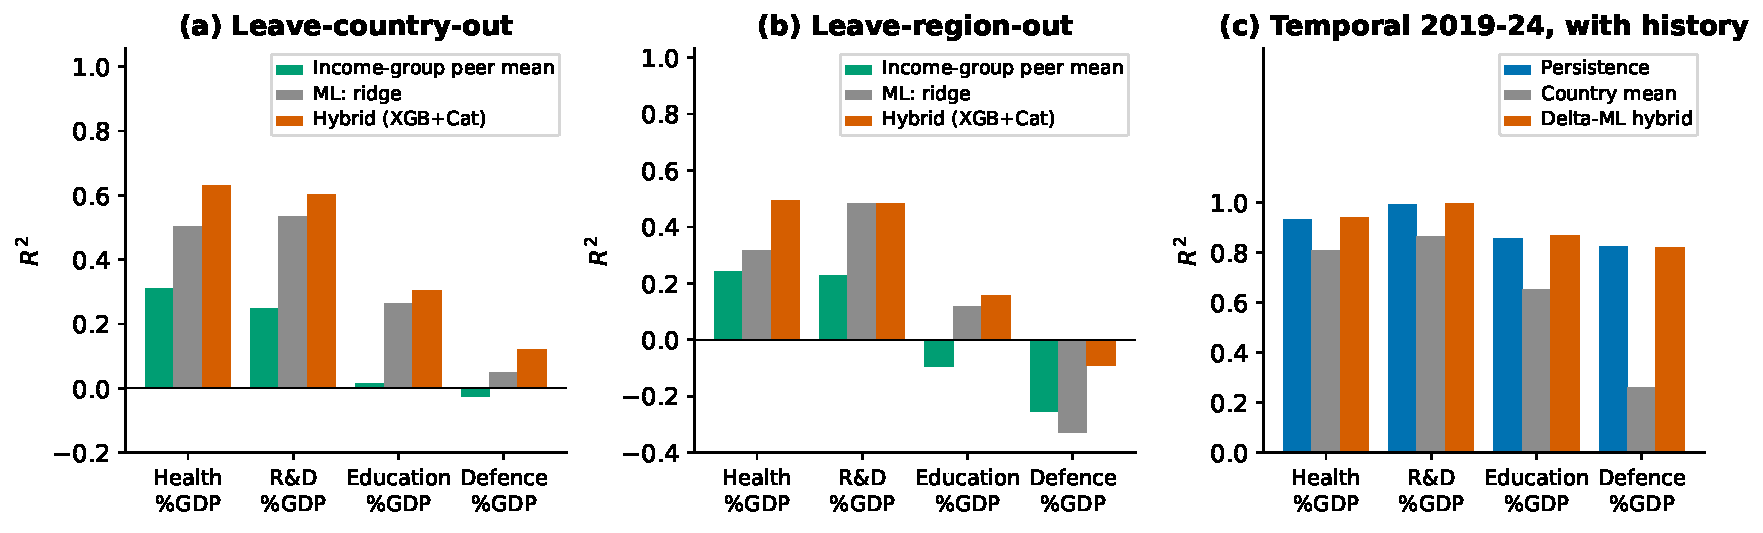
\includegraphics[width=\textwidth]{figures/fig6_wdi_panel.pdf}
\caption{Global WDI panel (one fold seed): $R^2$ for four official functions under (a) leave-country-out, (b) leave-region-out and (c) temporal evaluation.}\label{fig:wdi}
\end{figure}}
\newcommand{\figShap}{\begin{figure}[htbp]
\centering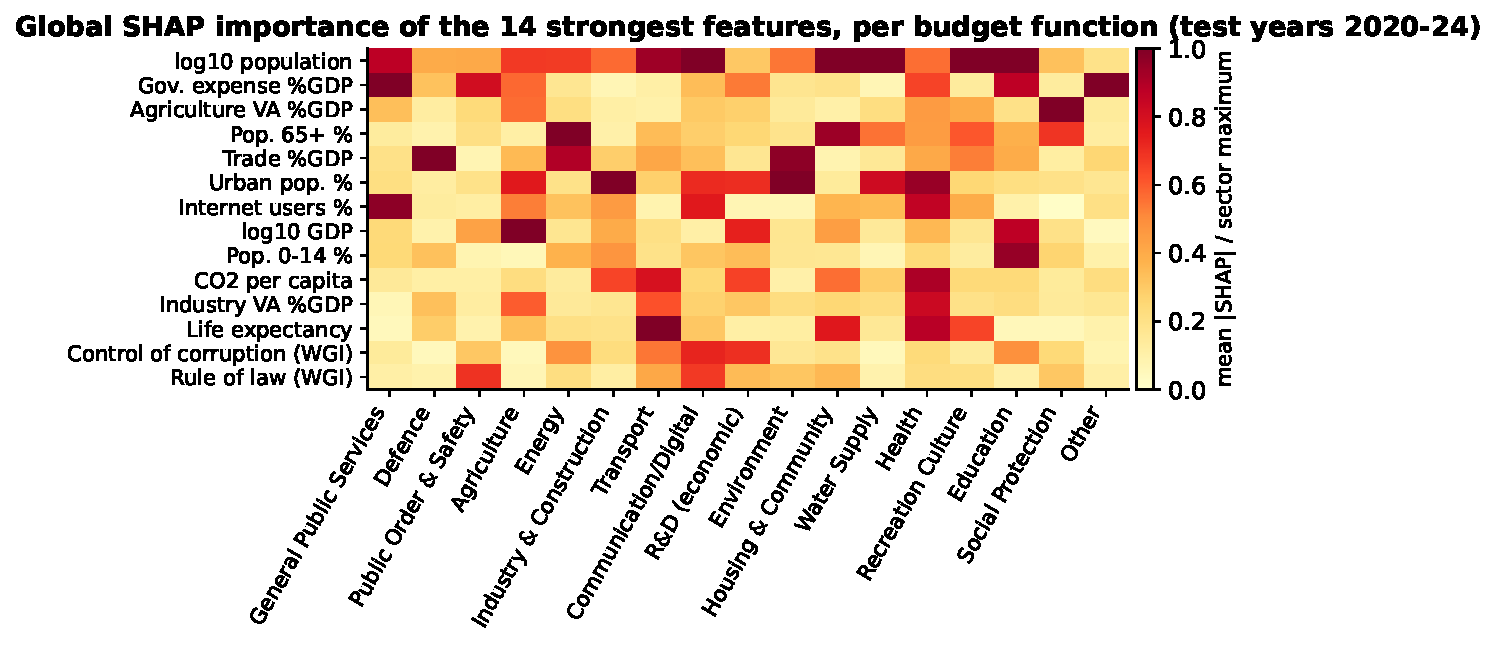
\includegraphics[width=0.9\textwidth]{figures/fig7_global_shap.pdf}
\caption{Global SHAP importance (mean $|\phi|$ normalised by each function's maximum) of the 14 strongest features for each budget function, test years 2020--24 (XGBoost member).}\label{fig:shap}
\end{figure}}
\newcommand{\figLime}{\begin{figure}[htbp]
\centering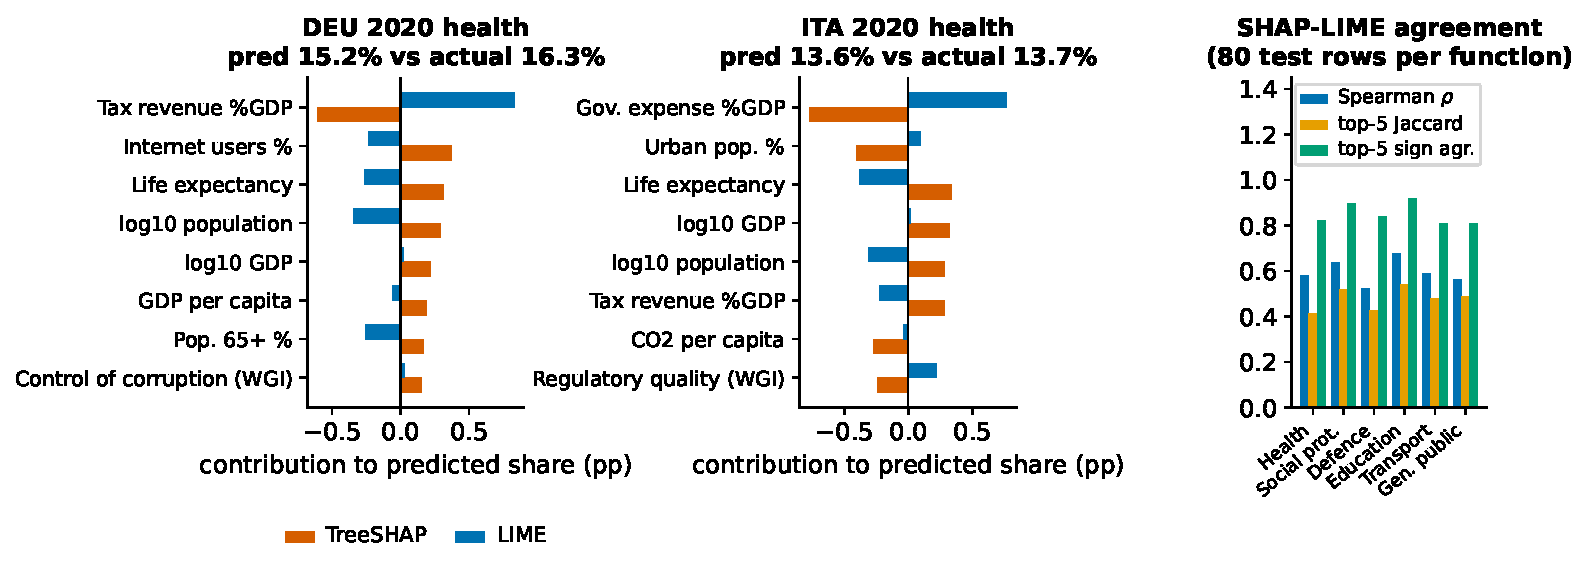
\includegraphics[width=\textwidth]{figures/fig8_shap_vs_lime.pdf}
\caption{SHAP vs.\ LIME. Left and centre: signed contributions for two test cases (feature values in Table~\ref{tab:features} units). Right: agreement metrics over 80 test rows per function.}\label{fig:lime}
\end{figure}}
\newcommand{\figWhatif}{\begin{figure}[htbp]
\centering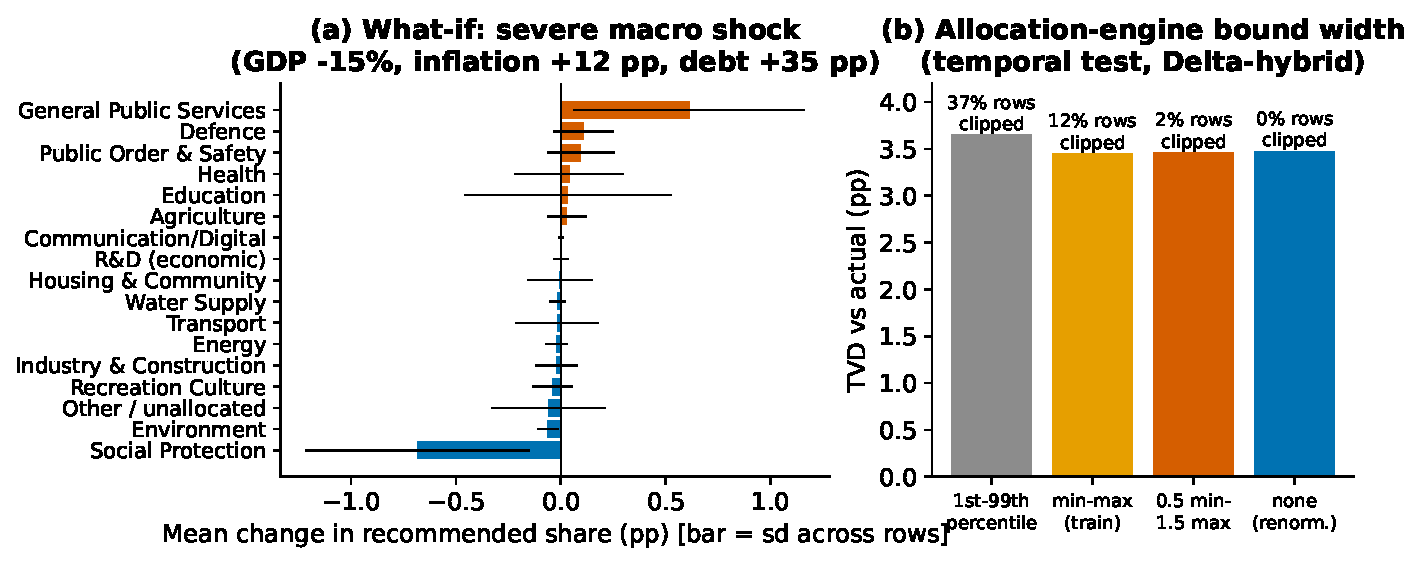
\includegraphics[width=\textwidth]{figures/fig9_whatif_engine.pdf}
\caption{(a) What-if sensitivity of the cold-start model to a severe macro shock (a model sensitivity, not a forecast). (b) Allocation-engine error vs.\ width of policy bounds (y-axis from zero); labels give the share of predictions that were clipped.}\label{fig:whatif}
\end{figure}}
\newcommand{\figCovid}{\begin{figure}[htbp]
\centering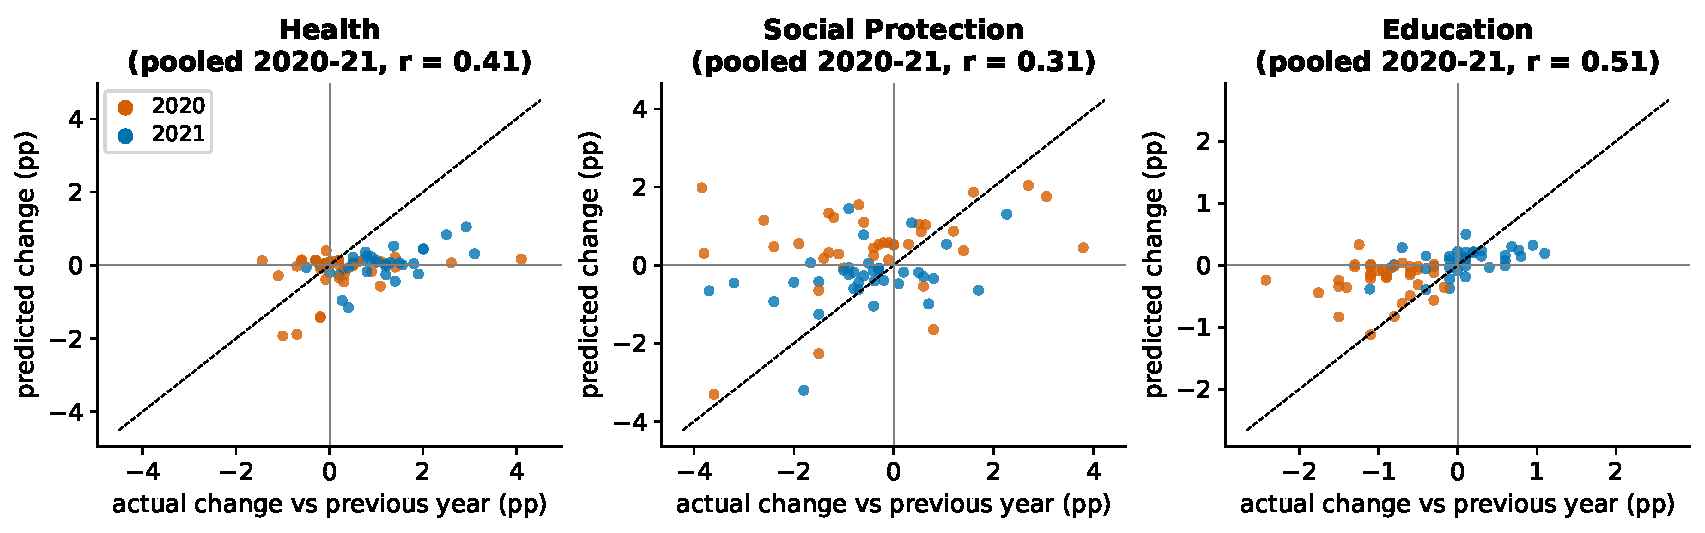
\includegraphics[width=\textwidth]{figures/fig10_covid_shift.pdf}
\caption{Predicted vs.\ observed one-year change in share, pooled 2020 and 2021 country-years (dashed line: perfect prediction); correlations are for the pooled points. The model captures the cross-country ranking only weakly and misses the aggregate shift.}\label{fig:covid}
\end{figure}}


\begin{document}
\begin{center}
{\LARGE\bfseries GovAllocXAI: A Benchmark of Explainable Machine Learning for Predicting Functional Government Expenditure Shares from Official Multi-Country Data\par}
\vspace{1.2em}
{\large Aditi H.\ Joshi$^{1,a,*}$, Pranav S.\ Chaudhari$^{1,b}$, Gaurav M.\ Jaypatre$^{1,c}$, Digvijay P.\ Birajdar$^{1,d}$\par}
\vspace{0.8em}
{\small\itshape $^{1}$Department of Computer Engineering, Pimpri Chinchwad College of Engineering, Pune, 411044, India\par}
\vspace{0.5em}
{\small $^{a}$aditi.joshi24@pccoepune.org; $^{b}$pranav.chaudhari24@pccoepune.org; $^{c}$gaurav.jaypatre24@pccoepune.org; $^{d}$digvijay.birajdar24@pccoepune.org\par}
{\small $^{*}$Corresponding author\par}
\end{center}
\vspace{0.6em}
\noindent{\color{linkblue}\Large\bfseries Abstract}\par\vspace{0.4em}
{\small\noindent How much can machine learning add to last year's government budget, and what can peers and explanations tell us when there is no last year? We build GovAllocXAI, an open benchmark for predicting how executed general-government expenditure is divided across COFOG functions. After finding that eleven of fifteen targets in our earlier semi-synthetic benchmark were exact multiples of one series, we rebuilt the evidence on official data: \NMasterRows{} country-year rows, COFOG shares for \NCofogCountries{} economies (\NTenEcon{} with IMF data) and World Bank sector series for \NWdiCountries{} economies. Under temporal, leave-country-out and leave-region-out protocols with cluster-bootstrap intervals, last year's allocation is a strong baseline (total-variation distance \ResTVDPersist{} pp). A learned correction using same-year covariates (a nowcast) lowers it to \ResTVDHyb{} pp, but the gain (\ResPairedGain{} pp, 95\% CI \ResPairedLo--\ResPairedHi) averages \AnnSeedMeanGain{} pp across learner seeds and is significant for only \AnnSeedNExcl{} of \AnnSeedN. Without history, a stacked learner and a nearest-economies average beat the income-group mean on the ten-division panel by about 1.3 pp (Holm-adjusted $p<0.001$) but not robustly on the 16-function panel; errors are two to three times larger for lower-income economies. Health and R\&D intensity are predictable in unseen economies ($R^2$ 0.63 and 0.60 vs.\ 0.31 and 0.25 for peers; ridge 0.50 and 0.53). SHAP and LIME agree more on direction (sign agreement \AgrSignMean) than on ranking (Spearman \AgrRhoMean). Data, code and the leakage audit are released.\par}
\vspace{0.5em}
\noindent{\small\textbf{Keywords:} government expenditure ; COFOG ; benchmark ; explainable AI ; SHAP ; LIME ; persistence baseline ; data leakage}
\vspace{0.8em}

\section{Introduction}\label{sec:intro}
Every government divides a limited budget among health, education, defence, social protection, transport and other functions. In practice the division is largely incremental: last year's allocation is adjusted for political priorities and expert judgment~\cite{davis1966,jones2005}. Machine learning (ML) can detect non-linear regularities in the socio-economic, fiscal and governance indicators that analysts cannot easily track jointly~\cite{athey2019,mullainathan2017}, and the allocations of comparable peer economies are rarely used systematically. Public-sector use, however, demands more than accuracy: a model output must be \emph{transparent}, and must remain an \emph{aid to, not a replacement for,} the accountable human decision-maker. This paper therefore asks a deliberately modest question: \emph{how much can machine learning add to last year's allocation, and what can peers and explanations tell us when there is no last year?}

\medskip\noindent\textbf{Use cases.} We see three defensible uses of such a model: (a) gap-filling and nowcasting of functional expenditure shares for statistical agencies and international organisations when official COFOG tables are late or missing; (b) peer benchmarking, i.e.\ showing what comparable economies typically spend; and (c) a benchmark dataset and protocol for research on compositional public-finance prediction. We do \emph{not} claim that the model tells a ministry what to allocate: the output is descriptive.

Existing ML work on public money mostly forecasts \emph{aggregate} expenditure as a time series~\cite{gur2025,dragulin2025}, predicts which projects or actors win competitive funds~\cite{caravaggio2025,distefano2025}, or relates spending to outcomes~\cite{valle2022,guerrero2022}. Studies of budgets by function or account group are few and mostly single-country~\cite{santschi2024,radulescu2015,nonato2026,mohith2026}, and explanation methods such as SHAP and LIME are rarely tested against each other or against known drivers. A further obstacle is data: no ready-made benchmark combines official functional spending with comparable macro-governance indicators across countries. Our own earlier version of this work (v1) used a semi-synthetic benchmark whose excellent scores turned out to be an artefact of the targets (Section~\ref{sec:audit}); the present paper replaces it with official data.

\medskip\noindent\textbf{Contributions.}
\begin{enumerate}
\item \textbf{An open, provenance-labelled dataset} (GovAlloc-COFOG~v1.0): \NMasterRows{} country-year rows for \NMasterCountries{} economies with \NFeatNum{} features, official COFOG functional allocations for \NCofogCountries{} economies (\NCofogRows{} complete country-years, 16 functions, Eurostat and OECD, cross-validated) and, with IMF data, ten COFOG divisions for \NTenEcon{} economies, plus official WDI sector series for \NWdiCountries{} economies; all legacy v1 columns are preserved.
\item \textbf{An evaluation protocol for compositional targets} with the baselines practitioners use (persistence, peer mean), temporal, leave-country-out and leave-region-out splits, a budget-reallocation metric (total-variation distance, TVD), cluster-bootstrap intervals and a Holm correction for the cold-start comparisons.
\item \textbf{A benchmark of learners and negative results:} boosted trees, a nested-NNLS stack, a nearest-economies predictor, Dirichlet regression, neural networks, econometric panel baselines, shock-aware and institutional features, evaluated against persistence and the income-group mean. Several components (a bounded-simplex projection and split-conformal intervals) are included as \emph{evaluated components}, not as proposed methods.
\item \textbf{A quantitative evaluation of SHAP and LIME} for this task (agreement, stability, fidelity, a deletion test and a synthetic ground-truth test).
\item \textbf{A forensic audit of our own earlier semi-synthetic benchmark} showing how $R^2>0.99$ arose from eleven sector columns that are exact multiples of one series.
\end{enumerate}
\medskip\noindent\textbf{Principal findings.} With official targets, last year's allocation is very hard to beat: a learned correction using same-year covariates reduces the share of budget to be moved from \ResTVDPersist{} to \ResTVDHyb{} percentage points for the pre-declared learner seed; the gain (\ResPairedGain{} pp) is small and not robust, averaging \AnnSeedMeanGain{} pp over five learner seeds with a 95\% interval that excludes zero for only \AnnSeedNExcl{} of \AnnSeedN{}. Without history, no learner significantly beats the income-group mean for the 16-function panel after multiple-comparison correction, whereas on the wider ten-division panel a stacked learner and a nearest-economies average each beat it by about 1.3 pp, and health and R\&D intensity are predictable in unseen economies ($R^2$ 0.63 and 0.60 vs.\ 0.31 and 0.25, although a plain ridge regression already reaches 0.50 and 0.53). SHAP and LIME agree on direction (top-5 sign agreement \AgrSignMean) more than on ranking (Spearman \AgrRhoMean), and attributions on correlated macro indicators are ambiguous. Errors are two to three times larger for lower-income economies. We argue that a clear statement of this competence map is more useful to analysts than a headline accuracy.

Throughout, the quantity predicted is the \emph{executed} (outturn) allocation of general-government expenditure across COFOG functions, the only quantity reported consistently across countries; it is not the approved budget appropriation, and we use ``allocation'' in this sense. The annual ``forecast'' is a \emph{nowcast}: it uses same-year covariates, which are realised values that are not known when a budget is drafted, whereas persistence uses only past information (Section~\ref{sec:method}).

The paper is organised as follows: Section~\ref{sec:related} reviews related work; Section~\ref{sec:data} describes the data; Section~\ref{sec:method} the models and protocol; Section~\ref{sec:results} the results; Section~\ref{sec:disc} discusses implications, threats to validity and governance; Section~\ref{sec:conc} concludes.


\section{Related Work}\label{sec:related}
\subsection{Machine learning for public budgets and expenditure}
Most work forecasts \emph{aggregate} public spending as a time series. G\"ur et al.~\cite{gur2025} compare machine- and deep-learning forecasters on T\"urkiye's monthly budget expenditure (2008--2024), including crisis periods; Dr\u{a}gulin et al.~\cite{dragulin2025} benchmark LSTM and TCN networks (among other models) against SARIMA, VAR and ECM; and Yang et al.~\cite{yang2023} forecast the government expenditure of 15 large economies with a GRU network and find it superior to ARIMA, ETS, SVR and XGBoost baselines. Barnes et al.~\cite{barnes2023} study empirically how OECD governments reallocate spending across COFOG functions (1996--2017) and find that countries with sounder governance and tighter fiscal rules reallocate more, but they build no predictive model. Nzazi et al.~\cite{nzazi2025} provide a narrative review of AI for public expenditure analysis in low-income countries and conclude that applications are mostly conceptual or pilot-scale. Santschi et al.~\cite{santschi2024} train XGBoost and CatBoost on Swiss cantonal accounts and study human--AI collaboration against expert forecasters (a short paper with preliminary results); the setting is one country and account groups rather than functional classes. R\u{a}dulescu et al.~\cite{radulescu2015} forecast public expenditure by function with feed-forward networks for five Central and Eastern European economies, before gradient-boosted trees became standard. Valle-Cruz et al.~\cite{valle2022} combine neural networks and a multi-objective genetic algorithm on 217 countries to relate expenditure strategies to outcomes such as inequality and growth and to explore how resources could be allocated; they do not predict an observed functional split.

\subsection{Funding allocation and public spending outcomes}
Caravaggio et al.~\cite{caravaggio2025} predict which actors win competitive EU rural-development funds; Di Stefano and Resce~\cite{distefano2025} uncover a need--allocation paradox in Italian recovery-plan calls; and Chand and Zhang~\cite{chand2022} study the gap between funding and expenditure in Australia's disability insurance scheme. These studies predict \emph{who} receives money at project or participant level, whereas we predict \emph{how a government budget is divided across functions}. On the outcome side, Guerrero and Casta\~neda~\cite{guerrero2022} propose a bottom-up causal framework linking spending to development gaps in 140 countries, and Nguyen et al.~\cite{nguyen2026} document a non-linear association between government expenditure and SDG progress. We use the SDGs only as a \emph{reporting} cross-walk from COFOG functions (Table~\ref{tab:sdg}; cf.\ the 2030 Agenda~\cite{un2015agenda}).

\subsection{Determinants and dynamics of public spending}
The public-economics literature studies why spending levels and mixes differ across countries and years. Government size has been analysed in the tradition of Wagner's law~\cite{lamartina2011}; the composition of public expenditure has been related to economic growth~\cite{devarajan1996,kneller1999,afonso2010}; globalisation, military-spending determinants and budget institutions have been examined as drivers of spending patterns~\cite{garrett2001,dunne2003,alesina1999}; and ideology and electoral cycles have been linked to the \emph{composition} of spending~\cite{potrafke2010,bove2017,nordhaus1975,rogoff1988,brender2005}. Budgeting has long been described as incremental~\cite{davis1966}, with occasional large punctuations~\cite{jones2005}; persistence as a hard-to-beat baseline is therefore the \emph{expected} result of this literature, and we test it rather than present it as a discovery. These studies are explanatory and use regressions on aggregates or a few categories; they do not provide out-of-sample prediction of the full functional composition. We add fiscal-rule, election and IMF-programme variables in one robustness module (Section~\ref{sec:ext}).

\subsection{Methodological background}
\textbf{Compositional targets.} Shares of a total are compositional data~\cite{aitchison1986}; log-ratio transformations~\cite{egozcue2003} and Dirichlet or beta regression~\cite{ferrari2004,douma2019} are the standard tools, and compositional methods have been applied to budget categories~\cite{adolph2020}. \textbf{ML in economics and forecasting.} Overviews of ML for economists~\cite{athey2019,mullainathan2017} and studies of ML for macroeconomic forecasting~\cite{medeiros2021,goulet2022} report that nonlinear learners can improve on standard benchmarks when data are rich, which motivates, but does not guarantee, gains on budget shares. \textbf{Trees versus deep learning on tabular data.} Tree ensembles remain strong on medium-sized tabular data~\cite{grinsztajn2022,shwartzziv2022,borisov2024}, and tabular deep models need careful design~\cite{gorishniy2021}; our panels are small, so we include an MLP and a feature-tokenising transformer only as comparators. \textbf{Uncertainty.} Split-conformal prediction gives distribution-free intervals under exchangeability~\cite{lei2018,angelopoulos2023}, and variants adapt the interval width to heteroscedasticity~\cite{romano2019}; coverage can fail when exchangeability fails~\cite{barber2023}, as it does when a new economy differs from the calibration economies. \textbf{Fairness.} Error that differs systematically between groups is an equity issue~\cite{mehrabi2021}; deployed prediction systems have been shown to under-serve disadvantaged groups~\cite{obermeyer2019}, and error-rate parity is one formal criterion~\cite{hardt2016}.

\subsection{Explainable AI in fiscal applications}
SHAP~\cite{lundberg2017,lundberg2020} and LIME~\cite{ribeiro2016} are routinely attached to gradient-boosted models in economics and public-sector studies, for instance for enterprise performance~\cite{zhang2026} or for patient-level health-insurance cost prediction~\cite{yao2025}. Such studies usually display attribution plots without testing whether the attributions are \emph{faithful, stable or consistent across methods}, although explainers are known to disagree with each other~\cite{krishna2022}, post-hoc explanations can be unstable~\cite{alvarezmelis2018,ghorbani2019}, manipulable~\cite{slack2020} and, in high-stakes settings, inferior to inherently interpretable models~\cite{rudin2019}; Shapley-value attributions have specific conceptual problems as importance measures~\cite{kumar2020}; and removal-based evaluations of attributions, which our deletion test resembles, have their own pitfalls~\cite{hooker2018,bhatt2020}. We follow the call for rigorous evaluation of interpretability~\cite{doshi2017} and report agreement, stability, deletion and ground-truth tests.

\subsection{Recent closely related studies (2025--2026)}
A web search in November 2026 (strings in the repository; a Scopus, Web of Science and IEEE Xplore search is still to be run) found five recent studies that touch our setting. Nonato et al.~\cite{nonato2026} predict Brazil's federal executed spending by budgetary function with a multi-output XGBoost and Bayesian optimisation; their series has 24 annual observations that they augment with 1\,048 synthetic points, they report $R^2$ up to 0.97 and a separate leakage-free check with much lower performance (we could verify the first figure but not the second from the accessible record). The study covers one country and does not use COFOG; as far as we can tell from the abstract it uses no explanation method. Kisman et al.~\cite{kisman2026} explain cross-country defence expenditure (2002--2023) with explainable-AI methods; it targets one function and an expenditure level rather than the composition of the whole budget. Dhungel et al.~\cite{dhungel2025} report an exploratory case study of AI decision support for budget preparation in Germany, and Francies et al.~\cite{francies2026} propose a SHAP, causal and counterfactual framework for urban budget allocation in smart cities (preprint). Mohith et al.~\cite{mohith2026}, known to us from the abstract only, benchmark classical and deep-learning models for one-year-ahead forecasts of India's Union-Budget allocations to twelve sectors (FY 2005--06 to 2024--25), find that gradient boosting and ridge regression beat the deep-learning models, and add SHAP, permutation importance, LIME and prediction intervals. Their finding that simple models win on short annual series agrees with ours, as does the caution about leakage in Nonato et al. What we add is scope and protocol: an \emph{official multi-country} COFOG panel with leave-country-out and temporal splits, persistence and peer baselines reported alongside every learner, a cluster-bootstrap and Holm-corrected comparison, and a test of the explanations rather than their display.

\subsection{Positioning}
We do not claim to be the first to predict budget allocations by ML, nor to propose a new learning method. Our contribution is the \emph{conjunction} of (i) an official, cross-validated multi-country functional-composition target, (ii) practitioner baselines and corrected inference, (iii) quantitative evaluation of SHAP and LIME on it, and (iv) an open audit of a leaky precursor benchmark. To the best of our (non-systematic) search no single prior study covers all four, but each is individually covered by some of the work above. Table~\ref{tab:gap} lists objective attributes of the closest studies; cells are filled from the full text where we read it and otherwise marked as judged from the abstract.

\begin{table*}[!t]
\caption{Closest prior work, described by objective attributes. Cells come from the full texts of Nonato, Kisman and Mohith and from the abstract of Francies; $^{\dagger}$ = judged from the abstract only. ``Explanations tested'' means that agreement, stability, faithfulness or ground-truth recovery of the attributions was quantified; ``shown'' means attributions were displayed.}\label{tab:gap}
\centering\footnotesize\setlength{\tabcolsep}{3pt}
\renewcommand{\arraystretch}{1.15}
\begin{tabular}{@{}p{2.7cm}p{3.1cm}p{2.7cm}p{2.3cm}p{1.9cm}@{}}
\toprule
\textbf{Study} & \textbf{Setting} & \textbf{Target} & \textbf{Explanation method} & \textbf{Explanations tested}\\
\midrule
G\"ur et al.~\cite{gur2025} & T\"urkiye, monthly 2008--2024 & aggregate expenditure & feature importance (TFT, RF, XGB, MLP) & no\\
Santschi et al.~\cite{santschi2024} & Switzerland, 26 cantons & account groups & none reported & no\\
R\u{a}dulescu et al.~\cite{radulescu2015} & 5 CEE countries & spending by function & none reported & no\\
Valle-Cruz et al.~\cite{valle2022} & 217 countries & spending vs outcomes & none reported & no\\
Guerrero \& Casta\~neda~\cite{guerrero2022} & 140 countries & spending vs SDG gaps & causal framework & n/a\\
Yao \& Zhu~\cite{yao2025} & patient-level insurance cost data & cost of care & SHAP & shown\\
Nonato et al.~\cite{nonato2026} & Brazil federal, 24 years (+ synthetic) & GDP growth, inflation, Gini given spending by function (allocation by optimisation) & none reported & no\\
Kisman et al.~\cite{kisman2026} & cross-country, 2002--2023 & classes of defence spending (share of GDP, share of spending, per capita) & SHAP, PDP, ALE & fidelity and faithfulness quantified\\
Mohith et al.~\cite{mohith2026} & India, 12 sectors, FY2005--2025 & absolute sector allocations (INR), one year ahead & SHAP, permutation, PDP, LIME (selected cases) & stability across two dataset variants\\
Francies et al.~\cite{francies2026}$^{\dagger}$ & Chicago and NYC municipal budgets, 2023--2026 & fund allocations & SHAP, causal model, counterfactuals & composite explainability score (fidelity, interpretability, equity)\\
\midrule
\textbf{This work} & \NCofogCountries{} / \NTenEcon{} economies (COFOG), \NWdiCountries{} (WDI), 2000--2024 & COFOG shares (16 / 10 functions), WDI sector series & TreeSHAP, LIME, KernelSHAP & agreement, stability, deletion, synthetic truth\\
\bottomrule
\end{tabular}
\end{table*}


\section{Data: GovAllocXAI-Data v2}\label{sec:data}
\subsection{Sources and provenance}
GovAlloc-COFOG~v1.0 is assembled exclusively from public, machine-readable official sources that were downloaded through their APIs (scripts in \texttt{pipeline/}; raw files kept verbatim in \texttt{data/raw/}):
\begin{itemize}
\item \textbf{World Development Indicators (WDI)}~\cite{wdi}: \NWdiIndicators{} indicators (GDP, population, inflation, unemployment, tax revenue, central-government debt, health and demographic indicators, infrastructure access, emissions, sector value added), plus four official sector-spending series: education, domestic general-government health, military and R\&D expenditure, each as share of GDP and (for the first three) of government expenditure.
\item \textbf{Worldwide Governance Indicators (WGI)}~\cite{kaufmann2011}: government effectiveness, control of corruption, rule of law and regulatory quality.
\item \textbf{Eurostat \texttt{gov\_10a\_exp}}~\cite{eurostat_cofog} and \textbf{OECD National Accounts Table~11}~\cite{oecd_table11}: general-government expenditure by function (COFOG~\cite{un2000cofog}), which provides the \emph{allocation targets}. OECD data are used only for economies absent from Eurostat (\NOecdAdded{} additional economies, \NOecdRowsComplete{} complete country-years); on the \NOverlapRows{}-row overlap the two sources agree to a median of \NXsrcMedDiff{}~percentage points (Pearson $r\ge \NXsrcMinR{}$ for all functions except communication, Section~\ref{sec:results}).
\item \textbf{IMF GFS expenditure by function}~\cite{imf_gfs}: general-government COFOG divisions (percent of total expenditure) for non-EU/OECD economies, used for the wide panel A10 and cross-checked against Eurostat (median difference $\le0.07$ pp on 723 overlapping country-years).
\end{itemize}
\figCoverage
\subsection{Structure of the released dataset}
The master table (\texttt{govallocxai\_v2\_master.csv}) has \NMasterRows{} rows (\NMasterCountries{} economies $\times$ 2000--2024, plus 25 legacy-only rows for Taiwan) and \NMasterCols{} columns: identifiers and country groupings, \NFeatNum{} features with a per-cell imputation flag, target series with source labels, and \emph{all columns of the legacy v1 dataset} (prefix \texttt{legacy\_}; country and year serve as keys) so that the earlier dataset is preserved and directly comparable. Two modelling panels are derived from it:
\begin{description}
\item[Panel A (COFOG; ``A16'' in the results).] \NCofogRows{} country-years from \NCofogCountries{} economies with a \emph{complete} 16-function breakdown. Targets are the share of total government expenditure (\%) of 16 functions: general public services, defence, public order and safety, agriculture, energy, industry and construction, transport, communication, R\&D (economic affairs), environment, housing and community amenities, water supply, health, recreation and culture, education and social protection, plus an explicit \emph{other/unallocated} residual so that the vector lies on the simplex (sums to 100\%). The 16 ``functions'' mix COFOG levels: general public services, defence, public order, environment, health, recreation, education and social protection are COFOG divisions; agriculture, energy, industry and construction (04.4 and 04.7), transport, communication and R\&D are groups of division 04 (economic affairs); water supply is group 06.3, and housing and community amenities is division 06 \emph{excluding} 06.3, so nothing is counted twice. The residual collects the remaining economic-affairs groups (general economic affairs 04.1 and 04.9 n.e.c.); it averages \ResidualMean\% of expenditure (median \ResidualMedian\%, maximum \ResidualMax\%) and is predicted and scored like a function.
\item[Panel A10 (wide COFOG).] \NTenRows{} country-years from \NTenEcon{} economies with a complete ten-division COFOG breakdown from Eurostat, OECD and IMF (priority in that order), including 35 middle- and low-income economies under the World Bank's \emph{current} classification, which is applied to all years. TVD values are not comparable between A16 (17 components) and A10 (10 components).
\item[Panel B (WDI).] \NWdiRows{} country-years from \NWdiCountries{} economies with at least one of the four official sector series (global coverage including low-income countries).
\end{description}
\subsection{Missing-value policy}
Targets are \emph{never} imputed. Features are filled in three ordered, flagged steps: (i) linear interpolation within a country series (maximum three consecutive years), (ii) edge fill (maximum three years), (iii) median of the region $\times$ income group $\times$ year cell. These steps are applied once to the whole table \emph{before} any cross-validation split, so interpolation can use later values and the cell medians pool all economies, including held-out ones; imputation is transductive and only features, never targets, are affected (Section~\ref{sec:disc}). Each imputed cell carries an \texttt{imp\_*} flag and each row an imputed-feature count. Features with high structural missingness (poverty headcount, Gini, adult literacy: 65--81\,\% of cells imputed) are \emph{excluded} from all models; \NFeatModel{} features remain (Table~\ref{tab:features}).
\subsection{Legacy dataset (v1)}
The v1 dataset (775 rows, 31 economies, 59 columns) is preserved verbatim. Its \emph{features} match the World Bank API values (exactly for GDP, population, life expectancy, growth, unemployment and internet use, and to within 0.4\% on 90\% of rows for inflation, on \NLegacyMatched{} matched rows), whereas its fifteen sector columns are mostly synthetic (Section~\ref{sec:audit}). v1 is therefore used only as an audited negative control, never as training evidence for the main results.


\section{Models and Evaluation Protocol}\label{sec:method}
\subsection{Problem formulation}
For economy $c$ and year $t$ let $\mathbf{x}_{c,t}\in\mathbb{R}^{p}$ be the socio-economic, fiscal, demographic and governance features, and let $\mathbf{y}_{c,t}=(y_1,\dots,y_{K})$ be the percentage shares of total general-government expenditure assigned to $K=17$ components (16 COFOG functions plus the residual; $K=10$ for panel A10), so that $y_k\ge 0$ and $\sum_k y_k=100$. The task is to learn $\hat{\mathbf{y}}_{c,t}=g(\mathbf{x}_{c,t},\mathbf{h}_{c,t})$ where $\mathbf{h}_{c,t}$ is optional history (last year's shares). The output is a descriptive reference for a human analyst, not a decision.

\textbf{Information set (nowcast, not forecast).} The features $\mathbf{x}_{c,t}$ are the \emph{same-year} values of GDP growth, inflation, debt and so on. These are realised values that are published with a lag and are not known when a budget for year $t$ is drafted; moreover, official COFOG for $t-1$ is itself published with a lag of 12--24 months. The annual regime below is therefore a \emph{nowcast} conditional on realised covariates, and persistence (which uses only $\mathbf{y}_{c,t-1}$) is evaluated on a less favourable information set than the learners. A strict forecast with lagged covariates was not run.

\figArch

\subsection{Prediction layer}
Two deployment regimes are distinguished because they correspond to different situations.
\paragraph{Regime~1: annual update with history.} The analyst knows last year's allocation $\mathbf{y}_{c,t-1}$. We learn the \emph{change}
\begin{equation}
\hat{\mathbf{y}}_{c,t}=\mathbf{y}_{c,t-1}+f\big(\mathbf{x}_{c,t},\mathbf{y}_{c,t-1}\big),
\end{equation}
so that persistence is the null model and the learner must earn any improvement.
\paragraph{Regime~2: cold start (no history).} For an economy without COFOG history, $\hat{\mathbf{y}}_{c,t}=f(\mathbf{x}_{c,t})$ is learned from \emph{other} economies; the benchmark is the mean allocation of the same World Bank income group (four classes).
\paragraph{Learners.} One regressor per component for XGBoost~\cite{chen2016xgboost}, LightGBM~\cite{ke2017}, CatBoost~\cite{prokhorenkova2018} and Random Forest~\cite{breiman2001}, and a ridge regression as a linear reference (hyper-parameters in Table~\ref{tab:hyper}; targets standardised before fitting). Tree ensembles are chosen because they are strong on medium-sized tabular data~\cite{grinsztajn2022}; our panels are smaller than those in that benchmark, so this is a prior, not a guarantee. The \emph{hybrid} is the equal-weight mean of XGBoost and CatBoost predictions, $\hat{\mathbf{y}}^{\text{hyb}}=\tfrac12(\hat{\mathbf{y}}^{\text{xgb}}+\hat{\mathbf{y}}^{\text{cat}})$; it is evaluated against its parts rather than assumed superior. Its choice was fixed before the test window was scored, but five learners and several variants were evaluated, so a best-of-several selection effect cannot be excluded.

\subsection{Further predictors evaluated}
\textbf{Log-ratio targets and stacking (architecture v2.1).} (i) \emph{History features:} lag-1 and lag-2 shares, their difference (trend) and the expanding mean of the country's \emph{past} shares. (ii) \emph{Compositional targets:} the centred log-ratio $\mathrm{clr}(\mathbf y)=\log(\mathbf y+\varepsilon)-\overline{\log(\mathbf y+\varepsilon)}$ with $\varepsilon=0.05$~\cite{aitchison1986,egozcue2003}, inverted by a softmax so that predictions are positive and sum to 100. (iii) \emph{Stacking}~\cite{wolpert1992}: for every component $k$ the final prediction is $\sum_m w_{m,k}\hat y^{(m)}_k$ with non-negative weights found by non-negative least squares and normalised to sum to one. In the annual mode the members are persistence, the past country mean and XGBoost/CatBoost learners (raw and log-ratio); weights are fitted on a validation window (train $\le$2016, validate 2017--19), the base models are refit on data up to 2019 and the test window is used once. In the cold-start mode the members are the peer mean, ridge, and XGBoost/CatBoost on log-ratio targets; weights come from a nested inner grouped cross-validation inside every outer training fold, so no test economy influences its weights.
\textbf{Nearest-economies predictor.} Features are median-filled and standardised with training economies only; each training economy is represented by the median of its feature vector over years; the query is compared with every training economy by Euclidean distance and the prediction is the inverse-distance-weighted average of the mean compositions of the $k$ nearest economies ($k=8$ in the comparisons; chosen from $\{3,5,8,12\}$ on out-of-fold data). Its neighbours are shown to the user, which makes it directly explainable.
\textbf{Dirichlet regression and neural networks.} An L2-penalised Dirichlet regression with concentration parameters $\alpha_k=\exp(\mathbf w_k^{\top}\mathbf x+b_k)$ on standardised features (a compositional model), a multilayer perceptron (five-seed ensemble, early stopping on an inner validation split of training economies) and a small feature-tokenising transformer~\cite{gorishniy2021} serve as comparators; both neural models predict softmax shares.
\textbf{Intervals (split conformal).} Absolute residuals per component are computed out-of-fold on the \emph{training} economies (inner grouped folds); their finite-sample $(1-\alpha)$ quantile~\cite{lei2018,angelopoulos2023}, either global or by income group (Mondrian variant), gives a symmetric band around each predicted share. Because out-of-fold residuals of grouped folds are not exchangeable with those of a genuinely new economy~\cite{barber2023}, nominal coverage is not guaranteed and is measured.
\textbf{Applicability score.} The mean standardised Euclidean distance of an economy's feature vector to its five nearest training economies; it is a novelty measure, not a probability.
\textbf{Econometric baselines.} A random walk with country drift, a pooled AR(1) on log-ratio shares with macro covariates, and the same with country fixed effects.

\subsection{Allocation engine (evaluated component)}
Raw predictions need not lie on the simplex or respect user-set limits. The engine first clips negatives and renormalises, then projects onto a bounded simplex:
\begin{equation}
\mathbf{a}^\star=\arg\min_{\mathbf{a}}\ \tfrac12\|\mathbf{a}-\hat{\mathbf{y}}\|_2^2\quad\text{s.t.}\quad \mathbf{1}^{\!\top}\mathbf{a}=100,\ \ \boldsymbol{\ell}\le\mathbf{a}\le\mathbf{u}.
\end{equation}
This is a standard Euclidean projection with solution $\mathbf{a}^\star=\operatorname{clip}(\hat{\mathbf{y}}+\lambda\mathbf{1},\boldsymbol{\ell},\mathbf{u})$ and scalar $\lambda$ found by bisection; we verify it against SLSQP (maximum discrepancy \NSlsqpDiff{} pp), which is a unit test rather than a result. The bounds $\boldsymbol{\ell},\mathbf{u}$ are set from training-data quantiles or minimum/maximum and are where statutory minima would be entered; no statutory constraints are available in our data, so we only study how bound width affects error (Section~\ref{sec:engine}).

\subsection{Explainability layer}
\textbf{SHAP.} Exact TreeSHAP~\cite{lundberg2017,lundberg2020} attributions $\phi_{j}$ are computed for every component model of the XGBoost member; global importance is $\overline{|\phi_j|}$. KernelSHAP (30 held-out rows per division, a 30-centre k-means background of the training rows, 200 samples) is used to explain the stacked blend directly. \textbf{LIME.} Reference tabular LIME~\cite{ribeiro2016} with continuous (non-discretised) features, 1\,500 perturbations and a local ridge surrogate; the signed local contribution of feature $j$ is $w_j(x_j-\bar{x}_j)/s_j$ so that it is comparable with $\phi_j$. Because post-hoc explanations can be unstable or manipulated~\cite{alvarezmelis2018,slack2020} and are not causal, we \emph{measure} them: (i) \emph{agreement} (Spearman $\rho$ between $|\phi|$ and $|$LIME$|$, top-5 Jaccard overlap, sign agreement on the top-5 features); (ii) \emph{stability} (Spearman $\rho$ between two LIME runs with different seeds); (iii) \emph{local fidelity} (LIME surrogate $R^2$); (iv) a \emph{deletion test}: the mean absolute prediction change when the three most important features (by SHAP) are replaced by the training mean, relative to three random features; and (v) a \emph{synthetic ground-truth test} with known drivers. The deletion test uses mean replacement, which creates off-manifold inputs, and any reasonable importance ranking would be expected to pass it; we did not compare with permutation or gain importance.

\subsection{Evaluation protocol}
\textbf{Metrics.} The primary metric is the \emph{total-variation distance} $\mathrm{TVD}=\tfrac12\sum_k|\hat y_k-y_k|$ in percentage points: the share of the budget that would have to be moved to turn the prediction into the observed allocation. It is interpretable to practitioners, scale-free across countries, and a natural reallocation measure; it is \emph{not} a log-ratio (Aitchison) distance, which would weight small functions more and which we do not report. TVD is dominated by the large functions (social protection, health, general public services). With $K$ components, MAE equals $2\,\mathrm{TVD}/K$ exactly, so MAE is not reported separately; RMSE and, for the single-target WDI series, $R^2$ are given where informative. Persistence is the naive benchmark recommended for forecast comparison~\cite{hyndman2006}. \textbf{Splits.} (a) \emph{Temporal}: train 2000--2019, test 2020--2024, which contains the COVID-19 shock and the 2022 energy crisis (block-wise validation respects temporal dependence~\cite{roberts2017,bergmeir2018}); it is a single origin, and persistence is about 60\% worse there than in the 2017--19 validation window (3.62 vs.\ 2.26\,pp); (b) \emph{leave-country-out}: six folds with all years of a country held out, repeated with two fold seeds (five for the robustness study); (c) \emph{leave-region-out} on the WDI panel (Panel B uses one fold seed). \textbf{Uncertainty.} 95\,\% confidence intervals are cluster-bootstrap intervals that resample \emph{countries} (2\,000 draws; 10\,000 in the Holm study) because years within a country are not independent~\cite{cameron2008}; with few clusters (36 in A16; three low-income economies in A10) they are approximate. \textbf{Multiplicity.} The family of eight cold-start comparisons (four per panel) is corrected with the Holm step-down procedure~\cite{holm1979}; the temporal comparison is reported with an uncorrected interval and is not claimed to be significant. \textbf{Paired gain.} Gains are paired differences of row-level TVD, averaged over fold seeds where stated; ``fold-seed~0'' marks values computed on the first fold seed only. \textbf{Baselines.} Persistence, country mean, income-group peer mean (four classes), global mean and ridge; no region-by-income mean or GDP-per-capita regression baseline was run. \textbf{Leakage control.} No feature is a transformation of a target; the audit of the v1 data (Section~\ref{sec:audit}) follows the leakage taxonomy of~\cite{kaufman2012}. Remaining leakage-type issues (transductive imputation, features that are components of spending) are listed in Section~\ref{sec:disc}.

\paragraph{Implementation details.} All experiments ran on a 12-core CPU workstation without GPU, Python 3.13 with XGBoost 3.2, LightGBM 4.6, CatBoost 1.2, scikit-learn 1.8, SHAP 0.52, LIME, PyTorch 2.9 (CPU), pandas 2.2, NumPy 2.2 and SciPy 1.16. Fixed seeds (42; five fold seeds for the robustness study) make every table reproducible; hyper-parameters are listed in the supplementary tables and were not tuned on test folds (Optuna tuning, Section~\ref{sec:ext}, used nested grouped cross-validation inside training economies).


\section{Results}\label{sec:results}
Table~\ref{tab:summary} summarises what worked and what did not; the subsections give the evidence. Unless stated otherwise, TVD values are in percentage points of total expenditure, CIs are 95\% cluster-bootstrap intervals over economies, and ``A16'' and ``A10'' denote the 16-function and ten-division COFOG panels (Section~\ref{sec:data}).

\begin{table}
\caption{Summary of the evidence: what worked and what did not (gains are TVD reductions in percentage points; Holm $p$ from Table~\ref{tab:holm}).}\label{tab:summary}
\centering\footnotesize
\renewcommand{\arraystretch}{1.12}
\begin{tabular}{@{}p{3.3cm}p{6.9cm}p{2.9cm}@{}}
\toprule
\textbf{Question} & \textbf{Evidence} & \textbf{Verdict}\\
\midrule
Learned correction beats last year (A16, nowcast)? & Gain \ResPairedGain{} (CI \ResPairedLo--\ResPairedHi) for learner seed 42; five-seed mean \AnnSeedMeanGain{}, CI excludes 0 in \AnnSeedNExcl{} of \AnnSeedN{} seeds & small, not robust\\
Same, wide panel A10? & stack \HistStackTen{} vs persistence \HistPersistTen{} (significantly worse) & no\\
Peers help without history, A16? & stack \FSStackSixteenGain{} (Holm $p=$ \FSStackSixteenHolm); 8-nearest \FSKnnSixteenGain{} (Holm $p=$ \FSKnnSixteenHolm) & weak\\
Peers help without history, A10? & stack \FSStackTenGain{} and 8-nearest \FSKnnTenGain{} (Holm $p=$ \FSStackTenHolm); XGBoost \FSXgbTenGain{} (Holm $p=$ \FSXgbTenHolm) & yes, modest ($\approx$8\% of a 15\,pp error)\\
Health and R\&D from indicators (WDI panel)? & $R^2$ 0.63 and 0.60 vs 0.31, 0.25 (peer mean); ridge 0.50, 0.53 & partly: mostly development level\\
Shock, institutional, WGI features; multi-year; econometric models? & none beats persistence or the baseline significantly & no\\
SHAP and LIME? & sign agreement \AgrSignMean, rank $\rho$ \AgrRhoMean; both recover 2 of 3 true drivers in a synthetic test & agree on direction, ambiguous for correlated features\\
Error by income group? & \ErrHigh{} (high) vs \ErrLow{} (low income, 3 economies) & worse for poorer economies\\
\bottomrule
\end{tabular}
\end{table}

\subsection{Forensic audit of the legacy benchmark}\label{sec:audit}
Before reporting new results we re-examine the legacy v1 benchmark, because its headline $R^2>0.99$ motivated this work. Three findings (Table~\ref{tab:audit}, Fig.~\ref{fig:audit}):
\begin{enumerate}
\item \textbf{One latent series, identical mix among eleven sectors.} Eleven of the fifteen sector columns are exact fixed multiples of one another (relative to agriculture: infrastructure $2.0\times$, social welfare $3.0\times$, transport $1.5\times$, energy $1.25\times$, housing $1.125\times$, rural development and industry $0.875\times$, water $0.75\times$, environment $0.625\times$, digital $0.5\times$; standard deviation of every ratio $\approx10^{-12}$). Among these eleven sectors all 775 country-years therefore share the same mix; only their total ($\approx16.7\%$ of GDP, CV 2.8\%, correlated $r=0.84$ with GDP growth) varies. There is no allocation pattern to learn in them; the other four sectors (defence, R\&D, education, health) do vary.
\item \textbf{GDP explains the $R^2$.} On these eleven sectors the one-parameter rule $k\times$GDP attains $R^2=\LegFormulaRConst$ versus $\LegXGBRConst$ for XGBoost on a random 80/20 split (USD scale), and a constant share of GDP gives $R^2=\LegConstRatioConst$ on the share scale. The mean over all fifteen sectors, $R^2=\LegXGBR$, is thus dominated by scale.
\item \textbf{Leakage and duplicated columns.} The legacy health-spending column is identical to the input feature of the same name (removing the feature changes $R^2$ from \LegHealthWith{} to \LegHealthWithout{} because other features still encode GDP), and \LegNIdent{} column pairs are identical, including all SDG ``budgets'' with their parent sector; the SDG-aligned model is therefore not an independent result.
\end{enumerate}
Only four legacy columns carry real information: education and R\&D equal the official WDI series (difference $<10^{-9}$ pp) and defence equals it to within 0.001\,pp (Pearson $r=0.998$), while healthcare differs from the official domestic government health series (median gap 2.4\,pp, $r=0.88$). The legacy \emph{features} match the World Bank values exactly for most indicators (inflation to within 0.4\% on 90\% of rows), which is why we keep and reuse them. With a temporal split on the legacy data XGBoost obtains $R^2=\LegTempXGB$ against \LegTempFormula{} for $k\times$GDP: again scale, not allocation. The legacy score therefore cannot support claims about learning budget-allocation patterns, and all conclusions below rest on official targets. The audit is a correction of our own earlier benchmark; we treat it as a methodological lesson on synthetic benchmarks, not as a main research result.

\begin{table*}
\caption{Forensic re-analysis of the legacy v1 benchmark (random 80/20 split as in the original notebooks). CV = coefficient of variation of sector/GDP across all 775 rows.}\label{tab:audit}
\centering\small
\renewcommand{\arraystretch}{1.1}
\resizebox{\linewidth}{!}{%
\begin{tabular}{rlcccccc}
\toprule
\# & Legacy sector & Mean \%GDP & CV (\%) & $R^2$ XGB (USD) & $R^2$ $k\!\times$GDP (USD) & $R^2$ XGB (share) & $R^2$ const. (share) \\
\midrule
1 & defence & 1.82 & 81.9 & 0.987 & 0.540 & 0.89 & $-$0.13 \\
2 & infrastructure & 2.47 & 2.8 & 0.999 & 1.000 & 0.95 & $-$0.00 \\
3 & research and development & 1.58 & 70.2 & 0.997 & 0.785 & 0.98 & $-$0.00 \\
4 & education & 5.43 & 79.4 & 0.978 & 0.823 & 0.76 & $-$0.03 \\
5 & healthcare & 7.31 & 44.3 & 0.987 & 0.709 & 0.98 & $-$0.00 \\
6 & agriculture & 1.24 & 2.8 & 0.999 & 1.000 & 0.91 & $-$0.00 \\
7 & rural development & 1.08 & 2.8 & 0.999 & 1.000 & 0.88 & $-$0.00 \\
8 & social welfare schemes & 3.71 & 2.8 & 0.999 & 1.000 & 0.96 & $-$0.00 \\
9 & energy & 1.54 & 2.8 & 0.999 & 1.000 & 0.93 & $-$0.00 \\
10 & transport & 1.85 & 2.8 & 0.999 & 1.000 & 0.93 & $-$0.00 \\
11 & housing and urban development & 1.39 & 2.8 & 0.999 & 1.000 & 0.92 & $-$0.00 \\
12 & water and sanitation & 0.93 & 2.8 & 0.999 & 1.000 & 0.85 & $-$0.00 \\
13 & environment and climate & 0.77 & 2.8 & 0.999 & 1.000 & 0.79 & $-$0.00 \\
14 & digital and IT & 0.62 & 2.8 & 0.999 & 1.000 & 0.70 & $-$0.00 \\
15 & industry and MSMEs & 1.08 & 2.8 & 0.999 & 1.000 & 0.88 & $-$0.00 \\
\bottomrule
\end{tabular}}
\end{table*}

\figAudit

\subsection{Annual update with history (Panel A16)}\label{sec:temporal}
Table~\ref{tab:A1} and Fig.~\ref{fig:main}a report the 2020--2024 test ($n=\ATest$ country-years; training: \ATrain{} country-years 2000--2019). \emph{Persistence is a strong baseline:} repeating last year's allocation requires moving only \ResTVDPersist\,pp of the budget (95\% CI \ResTVDPersistLo--\ResTVDPersistHi), compared with \ResTVDCountryMean\,pp for the country mean. This test window is hard: the same persistence rule misses by only 2.26\,pp in the 2017--19 validation window, so the COVID and energy-crisis years are about 60\% harder. Models that ignore history (features only) are clearly worse (6.3--9.2\,pp): a country's recent allocation carries far more information than its macro-indicators. The $\Delta$-learner (last year's shares plus a learned change) reduces TVD to \ResTVDHyb\,pp for the hybrid (CI \ResTVDHybLo--\ResTVDHybHi); for the pre-declared learner seed (42) the paired improvement over persistence is \ResPairedGain\,pp (95\% CI \ResPairedLo--\ResPairedHi, bootstrap over economies) and the hybrid is better on \ResRowsImproved\% of rows. This gain is \emph{small and not robust}: re-fitting the same hybrid with five learner seeds (42--46) gives gains of \AnnSeedMinGain--\AnnSeedMaxGain\,pp (mean \AnnSeedMeanGain\,pp) and a 95\% interval that excludes zero for only \AnnSeedNExcl{} of the \AnnSeedN{} seeds; XGBoost alone gains \AnnXgbSeedMeanGain\,pp on average and CatBoost provides most of the hybrid's gain. The individual learners (3.47--3.76\,pp) are statistically indistinguishable from the 50/50 hybrid, the log-ratio hybrid is indistinguishable from persistence (Section~\ref{sec:ext}), and this temporal comparison is not part of the Holm-corrected family. We therefore report the annual gain as a small positive point estimate that does not establish a reliable advantage over persistence. The learned change is informative about \emph{direction} for some functions (Fig.~\ref{fig:perfn}b: correlation 0.47 for education, 0.37 for general public services, 0.30 for health) but not for defence or R\&D (correlation $\approx0$).

\begin{table}
\caption{Temporal evaluation: train 2000--2019, test 2020--2024 ($n=178$ country-years, 36 economies); one-step-ahead with last year's allocation available. CIs: cluster bootstrap over economies. (MAE is omitted: with 17 components it equals TVD/8.5 exactly.)}\label{tab:A1}
\centering\small
\renewcommand{\arraystretch}{1.1}
\resizebox{\linewidth}{!}{%
\begin{tabular}{lccc}
\toprule
Method & TVD (pp) & 95\% CI & RMSE (pp) \\
\midrule
Persistence (last year) & 3.62 & [3.17, 4.08] & 0.923 \\
Country mean (train) & 6.96 & [6.16, 7.85] & 1.481 \\
Features-only: ridge regression & 9.22 & [8.37, 10.11] & 1.795 \\
Features-only: random forest & 6.45 & [5.72, 7.17] & 1.379 \\
Features-only: XGBoost & 6.64 & [5.94, 7.35] & 1.414 \\
Features-only: LightGBM & 6.34 & [5.68, 6.97] & 1.339 \\
Features-only: CatBoost & 6.44 & [5.78, 7.09] & 1.359 \\
Delta-learner: ridge regression & 3.76 & [3.31, 4.22] & 0.864 \\
Delta-learner: random forest & 3.47 & [3.04, 3.91] & 0.848 \\
Delta-learner: XGBoost & 3.59 & [3.15, 4.06] & 0.882 \\
Delta-learner: LightGBM & 3.63 & [3.17, 4.12] & 0.872 \\
Delta-learner: CatBoost & 3.50 & [3.08, 3.92] & 0.842 \\
Delta-learner hybrid (50\% XGBoost + 50\% CatBoost) & 3.48 & [3.06, 3.91] & 0.845 \\
\bottomrule
\end{tabular}}
\end{table}

\figMain

\textbf{COVID-19 and the energy crisis.} Fig.~\ref{fig:covid} compares predicted and observed one-year changes for 2020 and 2021. Models track the cross-country ranking of changes only weakly: for 2020 alone the correlation is \CovTwentyHealth\ for health and \CovTwentySocial\ for social protection, and for the pooled 2020--21 points in Fig.~\ref{fig:covid} it is \CovPooledHealth, \CovPooledSocial\ and \CovPooledEducation\ (health, social protection, education). They also miss the aggregate direction in 2020 (the mean health share rose by $+0.22$\,pp while the learned change was $-0.12$\,pp). Shock-year reallocations therefore remain the domain of human judgment.

\figPerfn
\figCovid

\subsection{Cold start: economies without history (Panel A16)}\label{sec:cold}\label{sec:selection}
In leave-country-out evaluation (Table~\ref{tab:A2}, Fig.~\ref{fig:main}b) the boosted hybrid reaches TVD \ResColdHyb\,pp (CI \ResColdHybLo--\ResColdHybHi) versus \ResColdPeer\,pp for the income-group peer mean and \ResColdGlobal\,pp for the global mean (two-seed means; the difference of the two means is $0.57$\,pp). The paired gain on fold-seed~0 only is \ResColdGain\,pp (95\% CI \ResColdGainLo\ to \ResColdGainHi), and the five-seed gain of single XGBoost is \FSXgbSixteenGain\,pp (CI \FSXgbSixteenLo\ to \FSXgbSixteenHi); neither is statistically significant, and ridge regression is worse than the peer mean. Composition across COFOG functions thus differs between economies for reasons the 25 macro-governance features capture only weakly (roughly one-tenth of the budget remains misallocated relative to the observed split). Note that the peer mean uses only four income classes and is the only simple baseline we ran; stronger simple baselines (region-by-income means, a GDP-per-capita regression) were not tested, and the ridge result suggests that linear baselines are also under-explored. Dropping any feature group raises error (Table~\ref{tab:ablation}; demographic/health indicators matter most) but all differences are within about two seed standard deviations. Richer feature specifications (region/income dummies, year-on-year changes) did \emph{not} help on a validation window and were not adopted (Table~\ref{tab:selection}).

\begin{table}
\caption{Cold-start evaluation: leave-country-out (6 folds, 2 fold seeds; TVD is the mean over both seeds), all 825 country-years, no history available.}\label{tab:A2}
\centering\small
\renewcommand{\arraystretch}{1.1}
\resizebox{\linewidth}{!}{%
\begin{tabular}{lccc}
\toprule
Method & TVD (pp) & 95\% CI & SD over fold seeds \\
\midrule
Hybrid (50\% XGBoost + 50\% CatBoost) & 10.77 & [9.60, 12.05] & 0.25 \\
random forest & 10.80 & [9.67, 12.07] & 0.12 \\
CatBoost & 10.83 & [9.65, 12.11] & 0.33 \\
XGBoost & 10.83 & [9.67, 12.12] & 0.16 \\
LightGBM & 10.97 & [9.79, 12.28] & 0.21 \\
Income-group peer mean & 11.34 & [10.33, 12.53] & 0.06 \\
Global mean & 11.35 & [10.35, 12.53] & 0.07 \\
ridge regression & 11.98 & [10.75, 13.26] & 0.18 \\
\bottomrule
\end{tabular}}
\end{table}


\subsection{Global evidence on four official functions (Panel B)}\label{sec:wdi}
The WDI panel (\NWdiCountries{} economies, 2000--2024) tests whether development indicators can predict the size of four official sector allocations in economies \emph{not} seen in training (Table~\ref{tab:B}, Fig.~\ref{fig:wdi}). In leave-country-out evaluation the hybrid explains $R^2=0.63$ of health spending (peer mean $0.31$) and $0.60$ of R\&D intensity (peer mean $0.25$); the gain is smaller for education ($0.30$ vs.\ $0.02$) and negligible for defence ($0.12$ vs.\ $-0.03$), whose level is driven by security context not captured by the features. A plain ridge regression already recovers most of this gain ($R^2$ 0.50 for health, 0.53 for R\&D), so the benefit of boosted trees over a linear model is modest ($+0.13$ and $+0.07$), and most of the advantage over the four-class peer mean reflects development level (GDP per capita). These targets are shares of GDP, whereas several features (central-government expense, tax revenue and debt, Table~\ref{tab:features}) describe the fiscal envelope from which the spending is financed; they are not transformations of the targets, but they are not independent of them either, and we did not re-run Panel B without them. Leave-\emph{region}-out is harder: health ($0.49$) and R\&D ($0.48$) remain predictable, education is weak ($0.16$), and defence and the shares-of-government-expenditure variants have \emph{negative} pooled $R^2$ under leave-region-out, so we caution against cross-region transfer for those functions. With history (temporal split), persistence is almost as good as the $\Delta$-hybrid ($R^2$ 0.93 vs.\ 0.94 for health, 0.86 vs.\ 0.87 for education, equal for defence and R\&D). Panel B is run with one fold seed, so no seed variability is reported.

\begin{table*}
\caption{WDI global panel, $R^2$. LCO = leave-country-out, LRO = leave-region-out: income-group peer mean vs.\ XGBoost+CatBoost hybrid. \emph{Temporal}: train $\le$2018, test 2019--2024, persistence vs.\ $\Delta$-hybrid with last-year value.}\label{tab:B}
\centering\small
\renewcommand{\arraystretch}{1.1}
\begin{adjustbox}{max width=\linewidth}
\begin{tabular}{lrcccccc}
\toprule
Official series & $n$ & LCO peer & LCO hybrid & LRO peer & LRO hybrid & Persist. & $\Delta$-hybrid \\
\midrule
Health (\%GDP) & 4547 & 0.31 & 0.63 & 0.24 & 0.49 & 0.93 & 0.94 \\
R\&D (\%GDP) & 2212 & 0.25 & 0.60 & 0.23 & 0.48 & 0.99 & 0.99 \\
Education (\%GDP) & 3365 & 0.02 & 0.30 & $-$0.10 & 0.16 & 0.86 & 0.87 \\
Defence (\%GDP) & 3814 & $-$0.02 & 0.12 & $-$0.25 & $-$0.09 & 0.82 & 0.82 \\
Health (\%gov. exp.) & 4547 & 0.28 & 0.43 & 0.25 & 0.14 & 0.89 & 0.90 \\
Education (\%gov. exp.) & 3304 & 0.06 & 0.13 & 0.02 & $-$0.13 & 0.78 & 0.78 \\
Defence (\%gov. exp.) & 3755 & 0.02 & 0.11 & $-$0.24 & $-$0.16 & 0.86 & 0.86 \\
\bottomrule
\end{tabular}\end{adjustbox}
\end{table*}

\figWdi

\subsection{Allocation engine (evaluated component)}\label{sec:engine}
The engine returns allocations that sum to 100\% to within $3\times10^{-14}$ and agree with an independent SLSQP solution to \NSlsqpDiff{} pp (maximum absolute difference, 100 rows). The width of the user-set bounds matters (Table~\ref{tab:bounds}, Fig.~\ref{fig:whatif}b): tight 1st--99th-percentile bounds clip 37\% of predictions and \emph{raise} error (TVD 3.65 vs.\ \EngTVDBefore\,pp without bounds) because \emph{observed} allocations frequently leave such narrow bands (43\% of test rows); bounds of $0.5\times$minimum to $1.5\times$maximum clip under 2\% of predictions with no accuracy loss. The projection is thus useful for enforcing the budget identity and for entering legal minima where they exist; it is not a mechanism to improve accuracy, and we do not count it as a methodological contribution.

\figWhatif

\subsection{Explainability}\label{sec:xai}
\paragraph{Global drivers.} Fig.~\ref{fig:shap} shows which features move each function's predicted share. Social protection is driven mainly by agriculture's value-added share (a proxy for development level) and the 65+ population share; education by population size, the 0--14 share and government expense; general public services by government expense, internet use and population; health by tax revenue, urbanisation, CO$_2$ per capita (a development proxy) and life expectancy; defence by trade openness. These are associations among correlated development indicators, not causal drivers, and the prominence of log population and government expense (the latter partly imputed, Table~\ref{tab:features}) shows that country size and fiscal-envelope variables enter the explanations.
\figShap
\paragraph{SHAP versus LIME (Table~\ref{tab:xai}, Fig.~\ref{fig:lime}).} Averaged over six functions, the rank correlation between $|\text{SHAP}|$ and $|\text{LIME}|$ is $\AgrRhoMean$, top-5 overlap (Jaccard) $\AgrJacMean$ and sign agreement on the top-5 features $\AgrSignMean$. The two methods therefore agree on \emph{direction} more than on \emph{ranking}; since a random sign has agreement 0.5 and most top features are monotone development proxies, part of the sign agreement is expected, and we did not compute a permuted-feature null. Individual cases can still disagree strongly: in the two case studies of Fig.~\ref{fig:lime} (Germany and Italy, health, 2020) the leading feature (tax revenue, respectively government expense, as \%GDP) has opposite signs under SHAP and LIME, because SHAP measures the contribution relative to the average prediction while LIME measures a local slope times the deviation from the mean, and attributions of correlated features can differ between the methods. A single explanation should therefore be read as a hypothesis. LIME local fits are modest ($R^2=\AgrLimeFit$ on average), and re-running LIME with another seed gives rank correlation $\AgrStabMean$ (0.75 for defence and general public services). In the deletion test, resetting the three most important SHAP features changes the prediction \AgrFaithMin--\AgrFaithMax$\times$ (mean \AgrFaithMean$\times$) as much as resetting three random features (six functions, 80 rows each). This shows that SHAP concentrates on features that move the model output; it is weak evidence of faithfulness because mean replacement creates off-manifold inputs and any importance ranking would be expected to pass, and we did not compare with permutation or gain importance. Neither method says that changing a feature would change a government's decision (Section~\ref{sec:disc}).
\begin{table*}
\caption{Quantitative evaluation of SHAP and LIME (80 random test rows per function). Faithfulness ratio = mean |prediction change| when the three most important SHAP features are reset to the training mean, divided by the same for three random features.}\label{tab:xai}
\centering\small
\renewcommand{\arraystretch}{1.1}
\begin{adjustbox}{max width=\linewidth}
\begin{tabular}{lcccccc}
\toprule
Function & Spearman $\rho$ & Top-5 Jaccard & Top-5 sign agr. & LIME local $R^2$ & LIME re-run $\rho$ & Faithfulness ratio \\
\midrule
Health & 0.58 & 0.41 & 0.82 & 0.47 & 0.92 & 3.1 \\
Social Protection & 0.64 & 0.52 & 0.90 & 0.59 & 0.92 & 3.4 \\
Defence & 0.52 & 0.43 & 0.84 & 0.56 & 0.75 & 3.4 \\
Education & 0.67 & 0.54 & 0.92 & 0.66 & 0.92 & 3.8 \\
Transport & 0.59 & 0.48 & 0.81 & 0.46 & 0.88 & 3.0 \\
General Public Services & 0.56 & 0.49 & 0.81 & 0.36 & 0.75 & 2.0 \\
\midrule
Mean & 0.59 & 0.48 & 0.85 & 0.52 & 0.86 & 3.1 \\
\bottomrule
\end{tabular}\end{adjustbox}
\end{table*}

\figLime
\paragraph{Synthetic ground truth.} In a synthetic test with known drivers (20 repetitions; one additive and one interaction term), TreeSHAP and LIME each recovered 2 of the 3 true drivers (precision@3 $=0.67$, identical in every repetition, i.e.\ a ceiling of two of three); when a near-copy of a driver was added, precision fell to 0.52 (TreeSHAP) and 0.43 (LIME) and attribution to the true driver dropped from 0.46 to 0.38 of the total. Correlated macro indicators therefore make single-feature attributions ambiguous, which is the setting of our real data.
\paragraph{What-if sensitivity.} Under a severe macro shock (GDP $-15\%$, inflation $+12$\,pp, debt $+35$\,pp; Fig.~\ref{fig:whatif}a) the cold-start model shifts shares by under 0.7\,pp for every function. General public services rises by 0.6\,pp (consistent with a larger debt-service burden) but social protection \emph{falls} by 0.7\,pp, contrary to the counter-cyclical expectation, because tree models cannot extrapolate beyond the support of the data and the shock moves several correlated features at once. Such scenarios are model sensitivities, not forecasts.

\subsection{Wider coverage (IMF data) and architecture v2.1}\label{sec:v21}
To test whether more and more diverse economies help, we added the IMF GFS expenditure-by-function dataset~\cite{imf_gfs} and built panel A10: the ten COFOG divisions for \NTenRows{} country-years of \NTenEcon{} economies, of which \NTenImf{} country-years (non-OECD economies such as India, Brazil, Indonesia) come from the IMF; on 723 overlapping country-years IMF and Eurostat agree to a median of at most 0.07\,pp (Pearson $r\ge0.984$ for all ten divisions). We also tested \emph{architecture v2.1}: history features, log-ratio targets and a non-negative least-squares \emph{stack} (Section~\ref{sec:method}).

\textbf{Annual update (Table~\ref{tab:Ehist}).} Neither richer history features nor log-ratio targets improve on the simple $\Delta$-learner. On panel A16 the stack (TVD \HistStackSixteen\,pp) is on par with the earlier hybrid and gains 0.11\,pp over persistence (paired, unrounded values; 95\% CI 0.03--0.20); on the wider panel A10 persistence is \HistPersistTen\,pp, the best learner \HistBestTen\,pp and the stack \HistStackTen\,pp: the stack is \emph{significantly worse} than persistence (paired $-0.20$\,pp, CI $-0.35$ to $-0.03$). For annual updates, persistence is the safer choice, and the simple $\Delta$-learner a marginal addition at best.

\textbf{Cold start (Tables~\ref{tab:Ecold} and~\ref{tab:holm}).} The stack has the lowest two-seed TVD on both panels. Averaged over five fold seeds, its paired gain over the income-group peer mean is \FSStackTenGain\,pp (95\% CI \FSStackTenLo--\FSStackTenHi, Holm-adjusted $p=$ \FSStackTenHolm) on A10 (TVD \FSTVDStackTen\ vs.\ \FSTVDPeerTen\,pp) and \FSStackSixteenGain\,pp (CI \FSStackSixteenLo--\FSStackSixteenHi, Holm $p=$ \FSStackSixteenHolm, not significant at 5\%) on A16 (\FSTVDStackSixteen\ vs.\ \FSTVDPeerSixteen\,pp). These are five-seed values and differ slightly from differences of the two-seed means in Table~\ref{tab:Ecold} (e.g.\ \ColdPeerTen{} $-$ \ColdStackTen{} $=1.24$ against 1.26). A single XGBoost gains \FSXgbTenGain\,pp (CI \FSXgbTenLo--\FSXgbTenHi) on A10 and \FSXgbSixteenGain\,pp on A16, neither surviving the Holm correction (the uncorrected A10 interval excludes zero), and the stack's advantage over XGBoost does not survive either. More, and more diverse, economies thus make peer learning useful on the wide panel, but the gain is about 1.3\,pp against an error of 15\,pp.

\begin{table}
\caption{Architecture v2.1, cold start (leave-country-out, 6 folds; TVD and CI are means over 2 fold seeds): peer mean, single learners (raw or log-ratio targets) and the nested-NNLS stack. Paired gains over the peer mean in the text are five-seed values (Table~\ref{tab:holm}), so they differ slightly from differences of the two-seed means shown here.}\label{tab:Ecold}
\centering\small
\renewcommand{\arraystretch}{1.1}
\begin{adjustbox}{max width=\linewidth}
\begin{tabular}{llcc}
\toprule
Panel & Method & TVD (pp) & 95\% CI \\
\midrule
A16 (36 economies) & Stack (nested NNLS) & 10.53 & [9.48, 11.67] \\
A16 (36 economies) & CatBoost (log-ratio targets) & 10.82 & [9.69, 12.04] \\
A16 (36 economies) & XGBoost (raw targets) & 10.83 & [9.67, 12.12] \\
A16 (36 economies) & XGBoost+CatBoost hybrid (log-ratio) & 10.86 & [9.72, 12.10] \\
A16 (36 economies) & XGBoost (log-ratio targets) & 11.07 & [9.91, 12.35] \\
A16 (36 economies) & Income-group peer mean & 11.34 & [10.33, 12.53] \\
A16 (36 economies) & Ridge & 11.98 & [10.75, 13.26] \\
\midrule
A10 (85 economies) & Stack (nested NNLS) & 13.77 & [12.30, 15.45] \\
A10 (85 economies) & XGBoost (raw targets) & 14.12 & [12.62, 15.78] \\
A10 (85 economies) & CatBoost (log-ratio targets) & 14.33 & [12.80, 16.13] \\
A10 (85 economies) & XGBoost+CatBoost hybrid (log-ratio) & 14.35 & [12.81, 16.13] \\
A10 (85 economies) & XGBoost (log-ratio targets) & 14.58 & [13.03, 16.34] \\
A10 (85 economies) & Ridge & 14.86 & [13.29, 16.70] \\
A10 (85 economies) & Income-group peer mean & 15.01 & [13.52, 16.80] \\
\bottomrule
\end{tabular}\end{adjustbox}
\end{table}

\begin{table}
\caption{Cold-start paired TVD gains averaged over five fold seeds, cluster bootstrap over economies (10\,000 draws), Holm correction over the family of eight comparisons. Positive = first method better.}\label{tab:holm}
\centering\small
\renewcommand{\arraystretch}{1.1}
\begin{adjustbox}{max width=\linewidth}
\begin{tabular}{llcccc}
\toprule
Panel & Comparison (cold start) & Gain (pp) & 95\% CI & Holm $p$ & Survives? \\
\midrule
A16 & Stack vs peer mean & 0.81 & [0.20, 1.34] & 0.060 & no \\
A16 & XGBoost vs peer mean & 0.47 & [-0.22, 1.13] & 0.171 & no \\
A16 & 8-nearest-economies vs peer mean & 0.66 & [0.19, 1.14] & 0.034 & yes \\
A16 & Stack vs XGBoost & 0.34 & [-0.03, 0.71] & 0.140 & no \\
A10 & Stack vs peer mean & 1.26 & [0.68, 1.84] & 0.0008 & yes \\
A10 & XGBoost vs peer mean & 0.89 & [0.19, 1.58] & 0.060 & no \\
A10 & 8-nearest-economies vs peer mean & 1.25 & [0.71, 1.78] & 0.0008 & yes \\
A10 & Stack vs XGBoost & 0.38 & [0.06, 0.69] & 0.060 & no \\
\bottomrule
\end{tabular}\end{adjustbox}
\end{table}


\textbf{Error by income group and applicability (Table~\ref{tab:income}).} Cold-start error rises steeply with income level: TVD \ErrHigh\,pp for high-income economies, 18.5 for upper-middle, \ErrLowerMid\ for lower-middle and \ErrLow\,pp for low-income economies, which have only nine and three training economies. An applicability score (Section~\ref{sec:method}) correlates with the error (Spearman $\rho=\NovRho$ over pooled rows), so the API reports it with every recommendation. This correlation is confounded by income group, which drives both novelty and error, and we did not compute a within-group partial correlation. Conclusions about low-income economies rest on three economies and are exploratory.

\begin{table}
\caption{Cold-start error (TVD, pp) by World Bank income group on the wide panel A10, with the mean applicability (novelty) score.}\label{tab:income}
\centering\small
\renewcommand{\arraystretch}{1.1}
\begin{adjustbox}{max width=\linewidth}
\begin{tabular}{lcccccc}
\toprule
Income group & Economies & Country-years & Novelty & Peer mean & Ridge & XGBoost \\
\midrule
High income & 50 & 1064 & 3.38 & 12.5 & 12.1 & 11.4 \\
Upper middle income & 23 & 371 & 4.05 & 18.3 & 19.4 & 18.5 \\
Lower middle income & 9 & 61 & 5.65 & 28.1 & 24.2 & 22.0 \\
Low income & 3 & 30 & 7.67 & 32.1 & 37.4 & 33.4 \\
\bottomrule
\end{tabular}\end{adjustbox}
\end{table}


\subsection{Total-budget module}\label{sec:total}
Shares become amounts only with a total. We therefore also model total general-government expenditure as a percentage of GDP (30 OECD/EU economies, 716 country-years with an observed total; the six OECD-only economies lack it) so that $\text{amount}_k=\text{share}_k\times\text{total}\times\text{GDP}$ (Table~\ref{tab:total}). In the temporal test a ridge $\Delta$-learner has a mean absolute error of \TotDeltaRidge\,pp of GDP against \TotPersist\,pp for persistence, because the 2020 shock moved total spending by several points of GDP and GDP growth is informative; for an economy without history the ridge model reaches \TotColdRidge\,pp against \TotColdMean\,pp for the group mean. Its feature set includes central-government expense as a percentage of GDP, which is a near-proxy for the target (correlation 0.75); in an internal audit check (not part of the released pipeline) dropping it raised the cold-start ridge error from 3.82 to 4.73\,pp, and dropping tax revenue, debt and expense together gave 5.97\,pp, worse than the group mean, so the module has no skill without those fiscal proxies. Because it is trained on OECD/EU economies only, its output for other economies is indicative; users may supply the total themselves.

\begin{table}
\caption{Total-budget module: general-government total expenditure as percent of GDP (30 OECD/EU economies, 716 country-years, Eurostat COFOG panel). MAE in percentage points of GDP. The income-group mean equals the global mean because all but one economy is high income.}\label{tab:total}
\centering\small
\renewcommand{\arraystretch}{1.1}
\resizebox{\linewidth}{!}{%
\begin{tabular}{llccc}
\toprule
Protocol & Method & $n$ & MAE (pp of GDP) & 95\% CI \\
\midrule
temporal 2020-24 & persistence & 150 & 2.87 & [2.57, 3.26] \\
temporal 2020-24 & country mean & 150 & 3.59 & [2.90, 4.49] \\
temporal 2020-24 & delta ridge & 150 & 1.83 & [1.62, 2.08] \\
temporal 2020-24 & delta xgb & 150 & 2.03 & [1.75, 2.38] \\
temporal 2020-24 & delta cat & 150 & 2.09 & [1.81, 2.43] \\
cold start leave-country-out & global mean & 716 & 5.63 & [4.47, 6.86] \\
cold start leave-country-out & income-group mean & 716 & 5.63 & [4.47, 6.86] \\
cold start leave-country-out & ridge & 716 & 3.82 & [3.13, 4.59] \\
cold start leave-country-out & xgb & 716 & 4.26 & [3.53, 5.02] \\
cold start leave-country-out & cat & 716 & 4.41 & [3.62, 5.24] \\
\bottomrule
\end{tabular}}
\end{table}


\subsection{Cold-start alternatives, intervals and fairness}\label{sec:ext}
\paragraph{Nearest economies.} The $k$-nearest-economies predictor ($k=8$, Section~\ref{sec:method}) is as accurate as the stack and XGBoost and is fully explainable: on A10 its five-seed TVD is 13.74\,pp against 14.11\,pp for XGBoost, and its gain over the peer mean is \FSKnnTenGain\,pp (CI \FSKnnTenLo--\FSKnnTenHi, Holm $p=$ \FSKnnTenHolm); on A16 the gain is \FSKnnSixteenGain\,pp (CI \FSKnnSixteenLo--\FSKnnSixteenHi, Holm $p=$ \FSKnnSixteenHolm). The value $k=8$ was fixed from a grid $\{3,5,8,12\}$ on out-of-fold data (where $k=12$ is marginally better) and the grid is not part of the Holm family, a mild forking-paths exposure. The API returns the five nearest economies with every recommendation.
\paragraph{Dirichlet regression and neural networks.} On the wide panel A10 the Dirichlet regression is as good as the stack (TVD 13.69\,pp against 13.77\,pp; 1.32\,pp better than the peer mean, CI 0.55--2.01) and the MLP reaches 13.85\,pp, whereas the transformer (14.14\,pp) matches XGBoost (14.08\,pp); on A16 none improves significantly on the peer mean or XGBoost. In the annual update no model beats persistence by a practically relevant margin (A10: best 4.58\,pp for a ridge $\Delta$-learner against 4.62\,pp; direct neural models without the persistence anchor are far worse, 6.55--6.91\,pp). A principled compositional model is therefore a strong, simple alternative to the stack for new economies, consistent with tree ensembles remaining strong on medium-sized tabular data~\cite{grinsztajn2022,shwartzziv2022}; our panels are smaller, so we read this only as a prior. (The stack, kNN and Dirichlet comparisons in this subsection and several below use fold-seed~0 or two-seed values, so the XGBoost cold-start TVD on A10 appears as 13.96 (fold-seed 0), 14.12 (two seeds) and 14.11\,pp (five seeds) in different tables; none changes a conclusion.)
\paragraph{Conformal intervals.} Split-conformal intervals calibrated on out-of-fold residuals of training economies reach near-nominal overall coverage (80\% $\to$ 80.1\%, 90\% $\to$ 90.3\%) but under-cover lower-income groups (low-income 47\%, lower-middle 61\% at the 80\% level), consistent with the lack of exchangeability discussed in Section~\ref{sec:method}; the website therefore warns users.
\paragraph{Hyper-parameter optimisation.} Optuna with nested grouped cross-validation on A10 gave no significant gain over the default settings (XGBoost 13.96 to 13.91\,pp, paired gain 0.05\,pp, CI $-0.19$ to 0.30; CatBoost 13.69 to 13.53\,pp, gain 0.17\,pp, CI $-0.09$ to 0.43; fold-seed 0), although the search was truncated by available compute; the defaults were kept.
\paragraph{Fairness by income group.} Cold-start error is largest for low-income economies (TVD \ErrLow\,pp against \ErrHigh\,pp for high-income). The max/min group ratio is 2.94 against 2.56 for the peer-mean baseline, so the learner does not close the gap for the lowest income group. The one detectable signed bias is an over-prediction of the social-protection share in low-income economies by 4.1\,pp. With three low-income economies, the bootstrap intervals for these quantities (23.7--40.9 for the error, 2.09--3.85 for the ratio, 2.5--7.0 for the bias) are not meaningful, and this audit is exploratory evidence of an equity concern rather than a formal fairness test.
\paragraph{Explaining the stacked blend.} Because the deployed recommendation is a blend, we also explained it directly with KernelSHAP (30 held-out country-years per division, panel A10) and compared it with TreeSHAP of the XGBoost member. The two explanations agree only moderately: the rank correlation of absolute attributions is 0.42 (health), 0.29 (education) and 0.37 (social protection), the top-5 overlap (Jaccard) is 0.32--0.39 and sign agreement on the top-5 features is 0.97, 0.71 and 0.77. KernelSHAP attributions on the blend change the blend 2.6, 1.3 and 2.8 times as much as random features when deleted. The explanation of the XGBoost member should therefore be read as indicative of, not identical to, the explanation of the blend.

\subsection{Negative results}\label{sec:neg}
\paragraph{Shock-aware features.} Growth, unemployment and debt changes, a recession dummy, a contemporaneous cross-country growth feature and a regime split did \emph{not} help: for 2020--21 on panel A16 the XGBoost shock-aware learner had TVD 4.16\,pp against 3.89\,pp for the baseline $\Delta$-learner (paired difference $-0.26$\,pp, 95\% CI $-0.41$ to $-0.11$) and 4.07\,pp for persistence; the CatBoost variant (4.01\,pp) was marginally below persistence but worse than its own baseline (3.73\,pp). In a global-financial-crisis hold-out (train up to 2007, test 2009--10) the XGBoost variant was likewise worse than persistence (4.07 vs.\ 3.43\,pp). Reallocation in crises remains a human judgment, in line with evidence on reallocation frictions~\cite{barnes2023}.
\paragraph{Multi-year projection.} Rolling origins (2012--19) and horizons of one to five years with recursive, frozen-macro and direct multi-horizon models: persistence was the best \emph{deployable} method at every horizon (A16: 2.92\,pp at $h=1$ and 5.63\,pp at $h=5$). A recursive projection with the \emph{true} future macro variables (an oracle) had TVD 2.80\,pp at $h=1$, a gain of 0.11\,pp over persistence that is not significant (CI $-0.13$ to 0.45), and was worse thereafter; frozen-macro projections were significantly worse. We do not offer multi-year projections.
\paragraph{Low-income coverage.} It cannot be repaired from the IMF source: its general-government COFOG file contains no values for 22 of 25 low-income and 35 of 47 lower-middle-income economies, and admitting central-government series with a relaxed consistency window adds only 13 country-years that are not comparable with general-government shares (mean TVD 7.5\,pp on the overlap). Inverse-frequency income weighting reduces low-income error only non-significantly (33.1 to 32.0\,pp).
\paragraph{Econometric panel baselines.} A random walk with country drift (TVD 3.73\,pp on A16, paired difference $-0.12$\,pp, CI $-0.15$ to $-0.09$), a pooled AR(1) on log-ratio shares with macro covariates (3.86\,pp) and the same with country fixed effects (3.88\,pp) are all significantly worse than repeating last year's allocation (3.62\,pp); on A10 the ordering is the same (persistence 4.62\,pp; 4.85--5.24\,pp for the econometric variants with penalty 1 and 4.63--5.0\,pp with penalty 10).
\paragraph{Robustness to fold seeds and multiple comparisons.} Table~\ref{tab:holm} gives five-seed gains with Holm correction over eight cold-start comparisons. Two claims survive at the 5\% level: the stack beats the income-group peer mean on A10 and the 8-nearest-economies predictor beats it on both panels. The stack on A16 ($p=0.060$), XGBoost over the peer mean ($p\ge0.06$) and the stack over XGBoost ($p\ge0.06$) do \emph{not} survive and should be read as suggestive. In the annual update, the log-ratio hybrid is statistically indistinguishable from persistence (raw $p=0.72$ on A16, $0.89$ on A10).
\paragraph{Institutional features.} Adding two keyless World Bank governance indicators (voice and accountability, political stability) and their two-year changes to the 25 features gave no significant gain: cold-start TVD 13.96 to 13.91\,pp (paired gain 0.04\,pp, CI $-0.12$ to 0.21) and, in the annual update, 4.74 to 4.71\,pp (gain 0.02\,pp, CI $-0.04$ to 0.08; 2020--21 only: 0.03\,pp). We then added three manually downloaded institutional sources: the IMF Fiscal Rules Dataset 1985--2024 (78\% of A10 rows covered), the Database of Political Institutions 2020 (election year and years to the next election; 77\%; ends in 2020) and the IMF MONA arrangements (programme active in the year; 100\%). Neither any single group nor all three together improved on the baseline. In cold start (three fold seeds) the paired gain (baseline minus extended TVD; negative means the extended model is \emph{worse}) was $-0.02$\,pp for fiscal rules (CI $-0.13$ to 0.09), $-0.02$\,pp for elections (CI $-0.09$ to 0.04), 0.00\,pp for IMF programmes (CI $-0.05$ to 0.06) and $-0.03$\,pp for all three (CI $-0.13$ to 0.08), i.e.\ TVD rose very slightly; in annual updates the gains were between $-0.016$ and $-0.006$\,pp with intervals that include zero (baseline 4.74\,pp). Institutional variables thus add no measurable predictive information beyond the economic, demographic and governance features already used, although coverage gaps (DPI ends in 2020) limit this conclusion.


\section{Discussion}\label{sec:disc}
\subsection{What the evidence supports}
(i) \textbf{As an annual predictor}, the learner adds at most a small, non-robust amount to persistence (\AnnSeedMeanGain\,pp on average over learner seeds, against a persistence error of \ResTVDPersist\,pp), and it is significantly worse than persistence on the wider panel; since it also uses same-year covariates (a nowcast), the honest reading is that last year's allocation is very hard to beat. (ii) \textbf{As a peer-informed prior}, it helps without history on the wide ten-division panel (about 1.3\,pp of a 15\,pp error, surviving Holm correction for the stack and the nearest-economies average), only weakly on the 16-function panel, and for health and R\&D intensity in the WDI panel, where a plain ridge regression already recovers most of the gain; it does not help for defence. (iii) \textbf{As an explanation device}, SHAP and LIME agree on direction more than ranking and both explain an association learned from peers, with ambiguity when macro indicators are correlated (synthetic test). (iv) \textbf{Under shocks}, the model reproduces neither the aggregate direction nor the magnitude of reallocation, so analyst judgment dominates. A system built on such a model should expose this competence map to its users. As a rule of thumb, the output is a \emph{reference point and prompt for questions} when an economy has no history, and at best a sanity check when last year's allocation exists.

\subsection{Intended use and human oversight}
The use cases (gap-filling, peer benchmarking, teaching) are descriptive. A cautious workflow would show last year's allocation first, the model reference as a peer benchmark, the gap in percentage points, and the nearest economies and attributions behind it; the analyst applies statutory bounds and records a rationale, and overrides are logged. The model must never auto-approve, and large gaps should prompt investigation, not correction: a model trained on past allocations reproduces past priorities and past biases. None of this has been tested with real users (Section~\ref{sec:open}).

\subsection{Threats to validity and limitations}
\textbf{Construct validity.} Targets are \emph{executed} general-government expenditure by COFOG function, not budget proposals; COFOG definitions are harmonised but practice differs between countries, the 16 ``functions'' mix COFOG levels (Section~\ref{sec:data}), and WDI sector series follow different definitions (e.g.\ UNESCO education, WHO health accounts) from COFOG. TVD weights large functions more; no log-ratio error is reported. \textbf{Information set.} The annual regime is a nowcast with realised same-year covariates; a strict forecast with lagged covariates, and publication lags of COFOG, were not modelled. \textbf{External validity.} The 16-function panel is OECD/EU-centred (high-income); the wide panel adds 35 middle- and low-income economies via the IMF, but only three are low-income, so low-income conclusions are exploratory. \textbf{Internal validity.} Hyper-parameters were fixed (or tuned within training economies) and a feature-specification choice was made on a validation window; nevertheless several comparisons are within sampling error, the temporal evaluation is a single origin dominated by COVID years, a best-of-several selection effect cannot be excluded for the annual hybrid, and with 36 clusters the intervals are wide and approximate. \textbf{Data handling.} Features (not targets) are imputed in three flagged steps \emph{before} cross-validation: interpolation can use later values and peer medians pool held-out economies, so imputation is transductive; the effect is likely small but was not measured, and fiscal features such as government expense (45.7\% imputed) and debt (69.3\%) are heavily affected (Table~\ref{tab:features}). The World Bank's \emph{current} income classification is applied to all years and is partly an outcome of the same economic history; it defines the peer-mean baseline and the group error tables. Some features (central-government expense, tax revenue, debt) are components of, or financed by, the spending envelope in Panel B and the total-budget module. \textbf{Baselines.} The peer mean has four classes; region-by-income and GDP-per-capita baselines were not run. \textbf{Explanations.} SHAP/LIME values depend on the background data and on correlated features; LIME is stochastic and its local fit is modest; the deletion test is weak; the explanations in the dashboard are for the XGBoost member, not the blend. \textbf{Deployment artefacts.} For an economy that is part of the training panel, the demonstration API returns in-sample fits (only the nearest-economies list excludes the queried economy), so its accuracy for such economies is higher than the leave-country-out errors reported here. \textbf{Non-stationarity.} Reallocation in crises (COVID-19, 2022 energy shock) is only weakly predicted.

\subsection{Governance, ethics and responsible use}
The tool is for \emph{assisting} analysts and for \emph{teaching} what peers allocate; it must not be used to justify cuts or to bypass legislative processes. Recommendations inherit the biases of historical budgets and of which economies publish COFOG data; errors are two to three times larger for lower-income economies, an equity concern that is documented but not resolved here~\cite{mehrabi2021,obermeyer2019}. No personal data are used. A model card and data sheet accompany the release; we recommend an independent audit before any operational use and a human-subject study of analyst use (future work).

\subsection{Reproducibility and data availability}
The processed panels, result files, scripts (\texttt{pipeline/01}--\texttt{27}) and \LaTeX{} sources are provided in the repository. The result macros, tables and figures of the manuscript are written by \texttt{pipeline/06b}, so those numbers cannot drift from \texttt{results/}; a few numbers in the running text are typed by hand from the same result files (fold-seed-0 values quoted in Section~\ref{sec:ext}, the legacy-audit statistics), and the internal audit check cited in Section~\ref{sec:total} is not part of the released pipeline. The dataset, code and manuscript sources are in the repository named in the Code availability statement.

\subsection{Which economies to include}
Holding out a whole region degrades or reverses performance for some functions (defence), cold-start error is two to three times larger for lower-middle- and low-income economies, which are under-represented, and the applicability score tracks this error. We therefore recommend training on all economies with official functional data, adding low-income economies as data become available, and reporting the applicability score so that users know when a reference is an extrapolation.

\subsection{Open items: human-subject evaluation}\label{sec:open}
All claims about supporting analysts remain untested with real users. A protocol, materials and analysis script for a three-condition between-subjects study (reference only; plus SHAP; plus SHAP, LIME and the applicability warning) are in the repository; running it requires ethics approval and about 160 participants for the primary comparison, which we leave to future work.


\section{Conclusion}\label{sec:conc}
We asked how much machine learning can add to last year's government allocation and what peers and explanations can tell us when there is no last year. On official COFOG data the answer is modest, and more informative than the legacy $R^2>0.99$ suggested: last year's allocation is a very strong baseline, and a learned correction using same-year covariates improves on it by only about \ResPairedGain{} percentage points of the budget for one learner seed (\AnnSeedMeanGain{} pp on average over five seeds, with an interval that excludes zero in \AnnSeedNExcl{} of \AnnSeedN); without history, a stack, a nearest-economies average and a Dirichlet regression beat the income-group mean by about 1.3 pp on the wide ten-division panel but not robustly on the 16-function panel; health and R\&D intensity are predictable in unseen economies, though a ridge regression gets most of the way there; shocks are not anticipated; errors are two to three times larger for lower-income economies; and SHAP and LIME agree on direction more than on ranking and are ambiguous when indicators are correlated. The stacked learner and the bounded-simplex projection are evaluated components, not recommended methods: the stack ties simpler alternatives and loses to persistence in annual mode. The released dataset, protocol, negative results and the audit that explains why an earlier benchmark looked better are, in our view, a more reliable contribution than a higher score.

\textbf{Future work.} (1) Strict forecasting with lagged covariates and publication lags, a rolling-origin evaluation of the headline comparison, and fold-internal imputation. (2) Extended COFOG coverage for non-OECD economies (IMF GFS, national treasuries; India's Union Budget as a case study) and stronger simple cold-start baselines. (3) Re-running Panel B without fiscal-envelope features, and permutation-importance and on-manifold deletion baselines for the explanations. (4) A curated library of statutory floors for the allocation engine. (5) Conformal intervals with group-conditional coverage guarantees for lower-income economies. (6) A human-subject study measuring decision time, agreement and trust calibration of analysts using the explanations.


\appendix
\section{Literature search protocol}
A web search was run on 14 November 2026 (not a systematic database search) with strings combining \emph{budget allocation / public expenditure}, \emph{machine learning / XGBoost / gradient boosting}, \emph{COFOG / functional classification}, \emph{SHAP / LIME} and \emph{SDG}. A repeat on Scopus, Web of Science and IEEE Xplore has not yet been run, and the novelty statement in Section~\ref{sec:related} is qualified accordingly. The query log and the closest papers are described in \texttt{docs/literature\_and\_novelty.md} of the repository; a later reference audit (Crossref and arXiv lookups of every cited DOI) is in \texttt{docs/audits/04\_reference\_audit.md}.

\FloatBarrier
\section{Supplementary tables}\label{app:tables}
\begin{table}[H]
\caption{The 25 model features (all from WDI/WGI; derived log transforms of GDP and population). Imputed-cell share is over the full master table.}\label{tab:features}
\centering\small
\renewcommand{\arraystretch}{1.1}
\begin{adjustbox}{max width=\linewidth}
\begin{tabular}{lllr}
\toprule
Feature & Group & Source & Imputed cells (\%) \\
\midrule
log10 GDP & Macro & WDI & 2.9 \\
log10 population & Demography & WDI & 0.0 \\
GDP per capita & Macro & WDI & 2.9 \\
GDP growth & Macro & WDI & 4.3 \\
Inflation & Macro & WDI & 16.1 \\
Urban pop. \% & Demography & WDI & 0.0 \\
Pop. 65+ \% & Demography & WDI & 0.0 \\
Pop. 0-14 \% & Demography & WDI & 0.0 \\
Tax revenue \%GDP & Fiscal & WDI & 43.2 \\
Central gov. debt \%GDP & Fiscal & WDI & 69.3 \\
Gov. expense \%GDP & Fiscal & WDI & 45.7 \\
Unemployment & Macro & WDI & 13.5 \\
Life expectancy & Health & WDI & 0.0 \\
Under-5 mortality & Health & WDI & 9.7 \\
Internet users \% & Development & WDI & 9.5 \\
Electricity access & Development & WDI & 1.3 \\
Basic water access & Development & WDI & 4.0 \\
CO2 per capita & Environment & WDI & 6.5 \\
Agriculture VA \%GDP & Structure & WDI & 9.9 \\
Industry VA \%GDP & Structure & WDI & 9.4 \\
Trade \%GDP & Structure & WDI & 17.5 \\
Gov. effectiveness (WGI) & Governance & WGI & 11.4 \\
Control of corruption (WGI) & Governance & WGI & 10.9 \\
Rule of law (WGI) & Governance & WGI & 9.6 \\
Regulatory quality (WGI) & Governance & WGI & 11.4 \\
\bottomrule
\end{tabular}\end{adjustbox}
\end{table}

\begin{table}[H]
\caption{Reporting cross-walk from COFOG functions to SDGs. It is a reporting layer chosen by the authors, \emph{not} a model input and not an official UN mapping.}\label{tab:sdg}
\centering\small
\renewcommand{\arraystretch}{1.1}
\begin{adjustbox}{max width=\linewidth}
\begin{tabular}{ll}
\toprule
COFOG function & Primary SDG(s) \\
\midrule
General Public Services & SDG~16 \\
Defence & SDG~16 \\
Public Order \& Safety & SDG~16 \\
Agriculture & SDG~2 \\
Energy & SDG~7 \\
Industry \& Construction & SDG~8, SDG~9 \\
Transport & SDG~9, SDG~11 \\
Communication/Digital & SDG~9 \\
R\&D (economic) & SDG~9 \\
Environment & SDG~13, SDG~15 \\
Housing \& Community & SDG~11 \\
Water Supply & SDG~6 \\
Health & SDG~3 \\
Recreation Culture & SDG~11 \\
Education & SDG~4 \\
Social Protection & SDG~1, SDG~10 \\
\bottomrule
\end{tabular}\end{adjustbox}
\end{table}

\begin{table}
\caption{Fixed hyper-parameters (no test-set tuning).}\label{tab:hyper}
\centering\small
\renewcommand{\arraystretch}{1.1}
\resizebox{\linewidth}{!}{%
\begin{tabular}{lp{9.5cm}}
\toprule
Model & Hyper-parameters \\
\midrule
XGBoost & 300 trees, lr 0.05, depth 3, subsample 0.8, colsample 0.8, min child weight 3, $L_2$ = 5 \\
LightGBM & 300 trees, lr 0.05, 8 leaves, min child 10, subsample 0.8, colsample 0.8, $L_2$ = 5 \\
CatBoost & 300 iterations, lr 0.07, depth 4, $L_2$ = 5 \\
Random Forest & 300 trees, min leaf 3, max features 0.5 \\
Ridge & $\alpha=10$, standardised inputs, median imputation \\
Hybrid & $0.5\,\hat{y}_{\text{XGB}}+0.5\,\hat{y}_{\text{Cat}}$ \\
All & targets standardised; seed 42; no tuning on test data (Section~\ref{sec:selection}) \\
\bottomrule
\end{tabular}}
\end{table}

\begin{table}[H]
\caption{Feature-spec selection on a validation window (train $\le$2016, validate 2017--2019; test years never used). In the cold-start regime richer specifications did not improve validation error. In the history regime the ``changes'' specification improved on the base specification (2.27 vs.\ 2.33\,pp) but remained worse than persistence (2.26\,pp); the base 25 features were kept.}\label{tab:selection}
\centering\small
\renewcommand{\arraystretch}{1.1}
\begin{adjustbox}{max width=\linewidth}
\begin{tabular}{llcc}
\toprule
Regime & Feature spec & \#features & Validation TVD (pp) \\
\midrule
history (delta learner) & BASE & 25 & 2.329 \\
history (delta learner) & PLUS\_groups & 31 & 2.373 \\
history (delta learner) & PLUS\_changes & 32 & 2.269 \\
history (delta learner) & PLUS\_both & 38 & 2.304 \\
history (delta learner) & persistence & 0 & 2.259 \\
cold-start features-only & BASE & 25 & 4.925 \\
cold-start features-only & PLUS\_groups & 31 & 4.970 \\
cold-start features-only & PLUS\_changes & 32 & 5.041 \\
cold-start features-only & PLUS\_both & 38 & 5.081 \\
\bottomrule
\end{tabular}\end{adjustbox}
\end{table}

\begin{table}[H]
\caption{Cold-start feature-group ablation (XGBoost, leave-country-out). Each row removes one group. SD is the population SD over the two fold seeds (ddof = 0), so it is not comparable with the sample SD in Table~\ref{tab:A2}.}\label{tab:ablation}
\centering\small
\renewcommand{\arraystretch}{1.1}
\begin{adjustbox}{max width=\linewidth}
\begin{tabular}{lccc}
\toprule
Feature set & \#features & TVD (pp) & SD over seeds \\
\midrule
all features & 25 & 10.83 & 0.12 \\
- governance (WGI) & 21 & 11.03 & 0.04 \\
- fiscal (tax, debt, expense) & 22 & 11.04 & 0.04 \\
- demographic/health & 20 & 11.14 & 0.28 \\
- macro (GDP, growth, inflation, trade) & 20 & 11.01 & 0.13 \\
- development/environment (internet, co2, water, structure) & 19 & 10.94 & 0.20 \\
\bottomrule
\end{tabular}\end{adjustbox}
\end{table}

\begin{table}[H]
\caption{Allocation-engine sensitivity to the width of the policy bounds (temporal test, $\Delta$-hybrid).}\label{tab:bounds}
\centering\footnotesize
\renewcommand{\arraystretch}{1.0}
\begin{adjustbox}{max width=\linewidth}
\begin{tabular}{lccc}
\toprule
Bounds & TVD (pp) & Predicted rows clipped (\%) & Actual rows outside (\%) \\
\midrule
1st-99th pctile & 3.649 & 37.1 & 43.3 \\
min-max (train) & 3.449 & 11.8 & 14.0 \\
0.5$\times$min - 1.5$\times$max & 3.464 & 1.7 & 3.4 \\
none (renorm only) & 3.476 & 0.0 & 5.6 \\
\bottomrule
\end{tabular}\end{adjustbox}
\end{table}

\begin{table}[H]
\caption{Architecture v2.1, annual update (one-step-ahead). Stack weights are fitted on the validation window; the test window 2020--24 is used once.}\label{tab:Ehist}
\centering\small
\renewcommand{\arraystretch}{1.1}
\begin{adjustbox}{max width=\linewidth}
\begin{tabular}{llccc}
\toprule
Panel & Method & Val. TVD & Test TVD & Test 95\% CI \\
\midrule
A16 & Persistence (last year) & 2.26 & 3.62 & [3.17, 4.08] \\
A16 & Country mean of past years & 5.25 & 6.59 & [5.86, 7.40] \\
A16 & Delta-learner: XGBoost & 2.33 & 3.59 & [3.15, 4.06] \\
A16 & Delta-learner: XGBoost + history features & 2.34 & 3.73 & [3.27, 4.21] \\
A16 & Delta-learner: CatBoost + history features & 2.27 & 3.62 & [3.19, 4.08] \\
A16 & Delta-learner: XGBoost, log-ratio + history & 2.39 & 3.78 & [3.25, 4.36] \\
A16 & Delta-learner: CatBoost, log-ratio + history & 2.35 & 3.71 & [3.24, 4.22] \\
A16 & Delta-learner hybrid, log-ratio + history & 2.33 & 3.69 & [3.21, 4.23] \\
A16 & Stack (NNLS on validation window) & 2.22 & 3.50 & [3.09, 3.93] \\
\midrule
A10 & Persistence (last year) & 3.26 & 4.62 & [3.93, 5.39] \\
A10 & Country mean of past years & 6.07 & 7.63 & [6.68, 8.75] \\
A10 & Delta-learner: XGBoost & 3.68 & 4.74 & [4.04, 5.49] \\
A10 & Delta-learner: XGBoost + history features & 3.55 & 4.71 & [4.00, 5.47] \\
A10 & Delta-learner: CatBoost + history features & 3.44 & 4.56 & [3.88, 5.28] \\
A10 & Delta-learner: XGBoost, log-ratio + history & 3.50 & 4.76 & [4.06, 5.52] \\
A10 & Delta-learner: CatBoost, log-ratio + history & 3.32 & 4.58 & [3.89, 5.32] \\
A10 & Delta-learner hybrid, log-ratio + history & 3.35 & 4.62 & [3.93, 5.37] \\
A10 & Stack (NNLS on validation window) & 3.34 & 4.82 & [4.13, 5.58] \\
\bottomrule
\end{tabular}\end{adjustbox}
\end{table}

\FloatBarrier

\section*{CRediT authorship contribution statement}
\begin{description}[leftmargin=!,labelwidth=5.2cm,itemsep=1pt,parsep=0pt]
\item[Conceptualization:] A.H.J., P.S.C.
\item[Methodology:] A.H.J., P.S.C., D.P.B.
\item[Software:] P.S.C., D.P.B.
\item[Validation:] G.M.J., D.P.B.
\item[Formal analysis:] P.S.C., G.M.J.
\item[Investigation:] G.M.J., A.H.J.
\item[Resources:] G.M.J.
\item[Data curation:] P.S.C., G.M.J.
\item[Writing -- original draft:] P.S.C., G.M.J.
\item[Writing -- review \& editing:] all authors
\item[Visualization:] D.P.B., P.S.C.
\item[Supervision and project administration:] A.H.J.
\end{description}
Author abbreviations: Aditi H.\ Joshi (A.H.J.), Pranav S.\ Chaudhari (P.S.C.), Gaurav M.\ Jaypatre (G.M.J.), Digvijay P.\ Birajdar (D.P.B.).

\section*{Declaration of competing interest}
All authors have reviewed the manuscript and declare that they have no known competing financial interests or personal relationships that could have appeared to influence the work reported in this paper.

\section*{Funding}
This research received no external funding.

\section*{Ethical approval}
This study is a secondary analysis of publicly released, aggregated national statistics (country-level government expenditure and macro-economic indicators). No human participants were recruited, no personal data were collected, and no institutional ethics approval was required. The human-subject evaluation described in the Discussion is future work and will require approval before it is run.

\section*{Declaration of generative AI and AI-assisted technologies in the manuscript preparation process}
During the preparation of this work the authors used Anthropic's Claude, an AI coding and writing assistant, for code scaffolding, data-collection scripts, drafting and editing of text, and for simulated critical review of the manuscript; the legacy v1 dataset analysed in Section~\ref{sec:audit} had itself been partly populated with the help of a large language model. References were checked with automated Crossref and arXiv lookups followed by manual correction. The authors reviewed and edited all content produced with these tools and take full responsibility for the content of the publication.

\section*{Data availability}
All inputs are public. World Development Indicators: \url{https://databank.worldbank.org/source/world-development-indicators}; Worldwide Governance Indicators: \url{https://www.worldbank.org/en/publication/worldwide-governance-indicators}; Eurostat \texttt{gov\_10a\_exp}: \url{https://ec.europa.eu/eurostat/databrowser/view/gov_10a_exp/default/table}; OECD National Accounts Table~11: \url{https://data-explorer.oecd.org/}; IMF Government Finance Statistics (COFOG): \url{https://data.imf.org/}. The harmonised panels (GovAllocXAI-Data v2.1, with provenance and imputation flags, and the preserved legacy v1 dataset) are in the \texttt{data/dataset\_new} folder of the repository below; a permanent Zenodo archive with a DOI is to be created at acceptance and its DOI inserted here. Redistribution of the derived panels follows the licences of the sources (World Bank CC BY 4.0; OECD, Eurostat and IMF terms of use).

\section*{Code availability}
All code (one script per pipeline stage, \texttt{pipeline/01}--\texttt{27}), the API and dashboard, the result files from which the numbers in this paper are generated, and the \LaTeX{} sources are in the public repository \url{https://github.com/Pranav-chaudhari-2006/GovAllocXAI-}.

\section*{Acknowledgements}
The authors thank the Department of Computer Engineering, Pimpri Chinchwad College of Engineering, Pune, for computing resources.

\bibliographystyle{IEEEtran}
\bibliography{references}
\end{document}
